
\documentclass[
  fontsize=10pt, % Base font size
  twoside=true, % Use different layouts for even and odd pages (in particular, if twoside=true, the margin column will be always on the outside)
  % open=any, % If twoside=true, uncomment this to force new chapters to start on any page, not only on right (odd) pages
  secnumdepth=1, % How deep to number headings. Defaults to 1 (sections)
  %chapterprefix=true, % Uncomment to use the word "Chapter" before chapter numbers everywhere they appear
  %chapterentrydots=true, % Uncomment to output dots from the chapter name to the page number in the table of contents
  numbers=noenddot, % Comment to output dots after chapter numbers; the most common values for this option are: enddot, noenddot and auto (see the KOMAScript documentation for an in-depth explanation)
  % draft=true, % If uncommented, rulers will be added in the header and footer
  % overfullrule=true, % If uncommented, overly long lines will be marked by a black box; useful for correcting spacing problems
]{kaobook}

% Choose the language
\usepackage[english]{babel} % Load characters and hyphenation
\usepackage[english=british]{csquotes}  % English quotes

% Load packages for testing
\usepackage{blindtext}
%\usepackage{showframe} % Uncomment to show boxes around the text area, margin, header and footer
%\usepackage{showlabels} % Uncomment to output the content of \label commands to the document where they are used

% Load the bibliography package
% \usepackage{styles/kaobiblio}
% \addbibresource{book-template.bib} % Bibliography file

% Load the package for hyperreferences
\usepackage{styles/kaorefs}

% Load mathematical packages for theorems and related environments. NOTE: choose only one between 'mdftheorems' and 'plaintheorems'.
\usepackage{styles/mdftheorems}
%\usepackage{styles/plaintheorems}

% \graphicspath{{images/}{./}} % Paths in which to look for images

\makeindex[columns=3, title=Alphabetical Index, intoc] % Make LaTeX produce the files required to compile the index

\makeglossaries % Make LaTeX produce the files required to compile the glossary

\makenomenclature % Make LaTeX produce the files required to compile the nomenclature



%----------------------------------------
% HL
%----------------------------------------

% \usepackage[backend=biber,natbib=true,maxcitenames=2,maxbibnames=10,giveninits=true,isbn=false,doi=false,url=false,defernumbers=true,style=numeric,sorting=ydnt]{biblatex} 
\usepackage[backend=bibtex,natbib=true,style=authoryear,citestyle=authoryear,maxcitenames=2,maxbibnames=10,giveninits=true,isbn=false,doi=false,dashed=false]{biblatex}
\bibliography{refs/3db} % Bibliography file
%-- remove the In:
\renewbibmacro{in:}{}
%-- remove the "" before/after the title of the paper
\DeclareFieldFormat[article, inbook, incollection, inproceedings, misc, thesis, unpublished]{title}{#1}



% Command to print a citation in the margins
\newcommand{\sidecitet}[1]{% The optional parameter is the 
%vertical shift; 
%the mandatory one is the citation key
  \citet{#1}% With this we print the marker in the text and add the item to the 
  %bibliography at the end \margincitation
  \marginnote{\citeauthor*{#1} (\citeyear{#1}), \citetitle{#1}\\}% 
  %Create a marginnote for each item
}

\newcommand{\sidecitep}[1]{% The optional parameter is the 
%vertical shift; 
%the mandatory one is the citation key
  \citep{#1}% With this we print the marker in the text and add the item to the 
  %bibliography at the end \margincitation
  \marginnote{\citeauthor*{#1} (\citeyear{#1}), \citetitle{#1}\\}% 
  %Create a marginnote for each item
}

\renewcommand{\ie}{ie}
\renewcommand{\eg}{eg}
% \newcommand{\reffig}[1]{Figure~\ref{#1}}
% \newcommand{\refsec}[1]{Section~\ref{#1}}
\newcommand{\refchap}[1]{Chapter~\ref{#1}}

\setcounter{margintocdepth}{1}
\setcounter{tocdepth}{1}

\usepackage{subcaption}
\usepackage{fontawesome}
\usepackage{boxedminipage}
\usepackage{gensymb}
\usepackage{listings}
\usepackage{color}
\definecolor{codegreen}{rgb}{0,0.6,0}
\definecolor{codegray}{rgb}{0.5,0.5,0.5}
\definecolor{codepurple}{rgb}{0.58,0,0.82}
\definecolor{backcolour}{rgb}{0.95,0.95,0.92}
\lstdefinestyle{mystyle}{
    backgroundcolor=\color{backcolour},   
    commentstyle=\color{codegreen},
    keywordstyle=\color{magenta},
    numberstyle=\tiny\color{codegray},
    stringstyle=\color{codepurple},
    basicstyle=\footnotesize,
    breakatwhitespace=false,         
    breaklines=true,                 
    captionpos=b,                    
    keepspaces=true,                 
    numbers=left,                    
    numbersep=5pt,                  
    showspaces=false,                
    showstringspaces=false,
    showtabs=false,                  
    tabsize=2
}
\lstset{style=mystyle,basicstyle=\ttfamily\footnotesize,breaklines=true}
\usepackage{xurl}
\usepackage{hyperref}
\hypersetup{breaklinks=true}

\setcounter{secnumdepth}{3}


%----------------------------------------------------------------------------------------

\begin{document}

%----------------------------------------------------------------------------------------
% BOOK INFORMATION
%----------------------------------------------------------------------------------------


\title{3D modelling of the built environment}
\author{Ken Arroyo Ohori \hspace{7mm} Hugo Ledoux \hspace{7mm} Ravi Peters}
\date{\texttt{v0.1}}

% \publishers{\includegraphics[width=\linewidth]{front-back/saba.png}}

%----------------------------------------------------------------------------------------

% \frontmatter % Denotes the start of the pre-document content, uses roman numerals

%----------------------------------------------------------------------------------------
% OPENING PAGE
%----------------------------------------------------------------------------------------

%\makeatletter
%\extratitle{
% % In the title page, the title is vspaced by 9.5\baselineskip
% \vspace*{9\baselineskip}
% \vspace*{\parskip}
% \begin{center}
%   % In the title page, \huge is set after the komafont for title
%   \usekomafont{title}\huge\@title
% \end{center}
%}
%\makeatother

%----------------------------------------------------------------------------------------
% COPYRIGHT PAGE
%----------------------------------------------------------------------------------------

% \input{front-back/pre}



%----------------------------------------------------------------------------------------
% OUTPUT TITLE PAGE AND PREVIOUS
%----------------------------------------------------------------------------------------

% Note that \maketitle outputs the pages before here

% If twoside=false, \uppertitleback and \lowertitleback are not printed
% To overcome this issue, we set twoside=semi just before printing the title pages, and set it back to false just after the title pages
% \KOMAoptions{twoside=semi}
% \maketitle
% \KOMAoptions{twoside=false}

%----------------------------------------------------------------------------------------
% PREFACE
%----------------------------------------------------------------------------------------

% \input{front-back/preface.tex}

%----------------------------------------------------------------------------------------
% TABLE OF CONTENTS & LIST OF FIGURES/TABLES
%----------------------------------------------------------------------------------------

\begingroup % Local scope for the following commands

% Define the style for the TOC, LOF, and LOT
%\setstretch{1} % Uncomment to modify line spacing in the ToC
%\hypersetup{linkcolor=blue} % Uncomment to set the colour of links in the ToC
\setlength{\textheight}{23cm} % Manually adjust the height of the ToC pages

% Turn on compatibility mode for the etoc package
\etocstandarddisplaystyle % "toc display" as if etoc was not loaded
\etocstandardlines % "toc lines as if etoc was not loaded

% \tableofcontents % Output the table of contents

% \listoffigures % Output the list of figures

% Comment both of the following lines to have the LOF and the LOT on different pages
% \let\cleardoublepage\bigskip
% \let\clearpage\bigskip

% \listoftables % Output the list of tables

\endgroup

%----------------------------------------------------------------------------------------
% MAIN BODY
%----------------------------------------------------------------------------------------

% \mainmatter 
\setchapterstyle{kao} % Choose the default chapter heading style

\setlength{\overflowingheadlen}{\linewidth}
\addtolength{\overflowingheadlen}{\marginparsep}
\addtolength{\overflowingheadlen}{\marginparwidth}
\renewpagestyle{scrheadings}{%
  {\hspace{-\marginparwidth}\hspace{-\marginparsep}\makebox[\overflowingheadlen][l]{%
    \parbox[t][1.7cm][c]{2em}{\hfill\thepage}%
    \makebox[2em][c]{\rule[-1.03cm]{1pt}{1.55cm}}%
    \parbox[t][1.7cm][c]{\textwidth}{\leftmark}}}%
  {\makebox[\overflowingheadlen][r]{%
    \parbox[t][1.7cm][c]{\textwidth}{\hfill\rightmark}%
    \makebox[2em][c]{\rule[-1.03cm]{1pt}{1.55cm}}%
    \parbox[t][1.7cm][c]{2em}{\thepage}}}%
  {\makebox[\overflowingheadlen][r]{%
    \parbox[t][1.7cm][c]{\textwidth}{\hfill\rightmark}%
    \makebox[2em][c]{\rule[-1.03cm]{1pt}{1.55cm}}%
    \parbox[t][1.7cm][c]{2em}{\thepage}}}%
}{%
  {}%
  {}%
  {}%
}
\renewpagestyle{plain.scrheadings}{
  {}%
  {}%
  {}
}{
  {\thepage}%
  {\parbox[t][0cm][c]{\overflowingheadlen}{\ccbysa\ Ken Arroyo Ohori, Hugo Ledoux and Ravi Peters. This work is licensed under a Creative Commons Attribution 4.0 International License (\url{http://creativecommons.org/licenses/by/4.0/})\newline(last update: \today)}}%
  {}
}
\pagestyle{scrheadings}
\newcommand*{\thelesson}{?.?}

% \include{dmds/dmds} % 1.1
% \include{brep/brep} % 1.2
% \include{voxels/voxels} % 2.1
% \include{LoD2recon/LoD2recon} % 2.2
% \include{dtvd3d/dtvd3d} % 3.1
% %!TEX root = ../3dchapter.tex
% chktex-file 46

\setchapterpreamble[u]{\margintoc}

\graphicspath{{iso19107/}}
\renewcommand*{\thelesson}{3.2}

\chapter{Three-dimensional geometries in geoinformation}%
\label{chap:iso19107}

To facilitate and encourage the exchange and interoperability of geographical information, the ISO (International Organization for Standardization: \url{www.iso.org}) and the OGC (Open Geospatial Consortium: \url{www.opengeospatial.org}) have developed in recent years standards that define what the basic geographical primitives are (the abstract specifications of ISO 19107), and also how they can be represented in a computer (the implementation specifications of GML and \emph{Simple Features}). 
While the abstract definitions for the primitives are not restricted to two dimensions (2D), most of the efforts for the representation and storage of the geographical primitives have been done only in 2D; the \emph{Simple Features} specifications are well-defined, used, and implemented across the GIS community.
\marginnote{Simple Features specifications}\index{Simple Features specifications}

This document gives an overview of the primitives in 3D, both from the ISO 19107 and the GML point-of-views.
Although the topic might appear trivial---``a polyhedron is simply a polyhedron, no?''---it is in practice a problem because several definitions exist and different software packages use different ones.
\marginnote{polyhedron}\index{polyhedron}

Having unambiguous definitions for the geometric primitives is important to foster interoperability, because most GIS operations (\eg\ calculation of the area of polygons; creation of buffers; conversion to other formats; Boolean operations such as intersection, union, etc.) require that the input primitives be according to certain definitions, otherwise the output of the operation is not guaranteed.

%%%
%
\section[Same polyhedra?]{Are your polyhedra the same as my polyhedra?}%
\label{sec:definition}

In the scientific literature, there is no single definition for a solid or a polyhedron (notice that these two terms are often used interchangeably).
Even in the field of mathematics, opinions differ as to what constitutes the term \emph{polyhedron}; many simply characterise the term as ``difficult to define''. 
Some researchers use it only for a regular polyhedron, or only for a convex one, and some consider non-planar faces as part of the definition.

%

The most common definition used is probably this simple one: a polyhedron is a 3D solid bounded by planar faces. 
The bounding faces are surfaces embedded in $\mathbb{R}^3$, the three-dimen\-si\-o\-nal Euclidean space, and together the bounding surfaces form a \emph{closed two-dimensional manifold} (or 2-manifold for short).
\marginnote{2-manifold}\index{2-manifold}
A 2-manifold is a topological space that is topologically equivalent to $\mathbb{R}^2$. 
An obvious example is the surface of the Earth, for which near to every point the surrounding area is topologically equivalent to a plane. 
An example of a 3-manifold is the entire Earth (its interior) because the neighbourhood of every point is equivalent to a sphere. 
\marginnote{3-manifold}\index{3-manifold}
The concept of neighbourhood, or locality, is such that a manifold can actually be constructed by `gluing' separate Euclidean spaces together.
Representing and storing a 2-manifold, even in $\mathbb{R}^3$, can be done with data structures that are intrinsically 2D since: (1) each edge is guaranteed to have a maximum of two incident faces; (2) around each vertex the incident faces form one `umbrella' (Figure~\ref{fig:nonmanifold}).
\begin{marginfigure}
  \centering
  \includegraphics[width=0.9\linewidth]{figs/nonmanifold}
  \caption{An example of an invalid 2-manifold: one edge and one vertex are non-manifold (the red ones).}%
\label{fig:nonmanifold}
\end{marginfigure}
The 2D data structures typically used in GIS, \eg\ the half-edge or the DCEL, can thus be used.



%%%
%
\section{The standard ISO 19107}

The geometric primitives as used in 3D GIS are based on the ISO 19107 definitions, and the definition of a polyhedra there is broader than that of a 2-manifold, to allow us to represent all the real-world features.

As shown in Figure~\ref{fig:isoprimitives}, 
\begin{marginfigure}
  \centering
  \includegraphics[width=\linewidth]{figs/isoprimitives.pdf}
  \caption{ISO 19017 primitives relevant for the modelling of the built environment.}%
\label{fig:isoprimitives}
\end{marginfigure}
the ISO 19107 geometric primitives for representing an object are: a 0D primitive is a \texttt{GM\_Point}, a 1D a \texttt{GM\_Curve}, a 2D a \texttt{GM\_Surface}, and a 3D a \texttt{GM\_Solid}.
A $d$-dimensional primitive is built with a set of $(d-1)$-dimensional primitives, \eg\ a \texttt{GM\_Solid} is formed by several \texttt{GM\_Surfaces}, which are formed of several \texttt{GM\_Curves}, which are themselves formed of \texttt{GM\_Point}.
Observe that the ISO19107 primitives do not need to be linear or planar, \ie\ curves defined by mathematical functions are allowed

%

In our context, the following three definitions from \citet{ISO19107} are relevant:
\begin{definition}
A \texttt{GM\_Solid} is the basis for 3-dimensional geometry. 
The extent of a solid is defined by the boundary surfaces.
The boundaries of \texttt{GM\_Solids} shall be represented as \texttt{GM\_SolidBoundary}.
[\ldots] 
The \texttt{GM\_OrientablesSurfaces} that bound a solid shall be oriented outward.
\end{definition}
\begin{definition}
A \texttt{GM\_Shell} is used to represent a single connected component of a \texttt{GM\_SolidBoundary}. 
It consists of a number of references to \texttt{GM\_OrientableSurfaces} connected in a topological cycle (an object whose boundary is empty). 
[\ldots] 
Like \texttt{GM\_Rings}, \texttt{GM\_Shells} are simple.
\end{definition}
\begin{definition}
A \texttt{GM\_Object} is \emph{simple} if it has no interior point of self-intersection or self-tangency. 
In mathematical formalisms, this means that every point in the interior of the object must have a metric neighbourhood whose intersection with the object is isomorphic to an $n$-sphere, where $n$ is the dimension of this \texttt{GM\_Object}.
\end{definition}

%

Observe that since shells (\texttt{GM\_Shell}s) are \emph{simple}, they are 2-manifold objects.
To be a valid shell, the 2-manifold should be closed, \ie\ there should not be `holes' in the surface (in other words, it should be watertight).
% It should furthermore be an orientable surface, Möbius strip not allowed.
% From Claus Nagel: However, the shell of a solid cannot be any 2-manifold, it must be a closed, orientable surface. Specifically, the shell must be homeomorphic to an n-holed torus, with the 0-holed torus being the n-sphere.

%

Figure~\ref{fig:onesolid} shows a solid that respects that definition.
\begin{marginfigure}
  \centering
  \includegraphics[width=0.95\textwidth]{figs/isosolid.pdf}
  \caption{One solid which respects the ISO 19107 definition. It has one exterior shell (grey) and one interior shell (orange) forming a cavity.}%
\label{fig:onesolid}
\end{marginfigure}
First observe that the solid is composed of two shells (both forming its boundaries), one being the exterior and one being the interior shell.
The exterior shell has eleven surfaces, and the interior one six.
An interior shell creates a cavity in the solid---cavities are also referred to as ``voids'' or holes in a solid.
A solid can have no inner shells, or several.
Observe that a cavity is not the same as a hole in a torus (a doughnut) such as that in Figure~\ref{fig:torus}: it can be represented with one exterior shell having a genus of 1\marginnote{The \textbf{genus} of an (orientable) surface embedded is the number of ``handles'' that it has. For instance, a doughnut and a mug have a genus of 1.} and no interior shell.
Observe also that the top face of the solid in Figure~\ref{fig:onesolid} has one inner ring, but that other surfaces ``fill'' that hole so that the exterior shell is closed.
\begin{marginfigure}
  \centering
  \includegraphics[width=0.8\linewidth]{figs/torus.pdf}
  \caption{A `squared torus' is modelled with one exterior boundary formed of ten surfaces. Notice that there are no interior boundary.}%
\label{fig:torus}
\end{marginfigure}


%%%
%
\section{Primitives used in practice}

\begin{figure}
  \centering
  \includegraphics[width=0.7\linewidth]{figs/geomprimitives.pdf}
  \caption{Some of the CityGML primitives, including aggregates and composites. Orange primitives are those representing inner boundaries. The \texttt{Shell} is not a class in GML, but it is implied when a \texttt{CompositeSurface} is used to define the boundary of a \texttt{Solid}.}%
\label{fig:geomprimitives}
\end{figure}

%

% TODO : chapter/lesson number
CityGML, the international standard for 3D modelling of cities (see Lesson~4.1), uses a subset of ISO 19107, with the following two restrictions: 
\begin{enumerate}
  \item \texttt{GM\_Curves} can only be \emph{linear} (thus only \texttt{LineStrings} and \texttt{LinearRings} are used); 
  \item \texttt{GM\_Surfaces} can only be \emph{planar} (thus \texttt{Polygons} are used).
\end{enumerate}

%

Following ISO 19107, in GML and CityGML geometric primitives can be combined into either \emph{aggregates} or \emph{composites}.

An aggregate (class \texttt{gml:\_AbstractGeometricAggregate}) is an arbitrary collection of primitives of same dimensionality that is simply used to bundle together geometries.
GML (and CityGML) has classes for each dimensionality (\texttt{Multi*}), the most relevant one in our context is \texttt{MultiSurface} that is often used in practice to represent the geometry of a building.
An aggregate does not prescribe any topological relationships between the primitives.

A composite of dimension $d$ is a collection of $d$-dimensional primitives that form a $d$-manifold. 
\marginnote{$d$-manifold}\index{$d$-manifold}
The most relevant example in our context is a \texttt{CompositeSurface}, which is a 2-manifold.



%%%
%
\section[Implementation specifications]{Implementation specifications for the 3D primitives}


Observe that for a primitive to be valid, all its lower-dimensionality primitives have to be valid.
For instance, a valid Solid cannot have as one of its surfaces a Polygon having a self-intersection (which would make it invalid).


%%%
\subsection{\texttt{Polygon}}

For a \texttt{Polygon} embedded in $\mathbb{R}^3$ to be valid, it needs to fulfil the 6 assertions in Figure~\ref{fig:ogcsf_definitions}, which are given on pages 27--28 of the OGC \emph{Simple Features} document.
These rules are verified by first projecting each \texttt{Polygon} to a plane, this plane is usually obtained by least-square adjustment of its points.
A \texttt{Polygon} must also be \emph{planar} to be valid: its points (used for both the exterior and interior rings) have to lie on a plane.
\begin{figure}
  \centering
  \begin{boxedminipage}{\textwidth}
    {\small
  \begin{enumerate}
    \item Polygons are topologically closed;
    \item The boundary of a Polygon consists of a set of LinearRings that make up its exterior and interior boundaries;
    \item No two Rings in the boundary cross and the Rings in the boundary of a Polygon may intersect at a Point but only as a tangent, \eg\
      \[
         \forall P \in Polygon, \forall c1, c2 \in P.Boundary(), c1 \neq c2,
      \]
      \[
          \forall p, q \in Point, p, q \in c1, p \neq q, [p \in c2 \Rightarrow q \notin c2];
      \]
    \item A Polygon may not have cut lines, spikes or punctures \eg:
      \[
         \forall P \in Polygon, P = P.Interior.Closure;
      \]
    \item The interior of every Polygon is a connected point set;
    \item The exterior of a Polygon with 1 or more holes is not connected. Each hole defines a connected component of the exterior.
  \end{enumerate}
  }
  \end{boxedminipage}
\caption{The six assertions for the validity of a 2D polygon, according to \emph{Simple Features}.}%
\label{fig:ogcsf_definitions}
\end{figure}



%%%
\subsection{\texttt{MultiSurface}}
It is an arbitrary collection of \texttt{Polygon}.
Validating a \texttt{MultiSurface} simply means that each \texttt{Polygon} is validated individually; a \texttt{MultiSurface} is valid if all its \texttt{Polygon}s are valid.


%%%
\subsection{\texttt{CompositeSurface}}
Besides that each \texttt{Polygon} must be individually valid, the \texttt{Polygon}s forming a \texttt{Composite\-Surface} are not allowed to overlap and/or to be disjoint.
Furthermore, if we store a \texttt{Com\-po\-site\-Surface} in a data structure, each edge is guaranteed to have a maximum of two incident surfaces (except those on the boundary), and around each vertex the incident faces form one ``umbrella'' (see Figure~\ref{fig:nonmanifold}).


%%%
\subsection{\texttt{Solid}}

According to ISO 19107, the different boundaries of a solid are allowed to interact with each other, but only under certain circumstances.
To understand these, we have to generalise to 3D the implementation specifications defined in 2D by the OGC (Figure~\ref{fig:ogcsf_definitions}).
Observe that all of them, except the third one, generalise directly to 3D since a point-set topology nomenclature is used.
The only modifications needed are that, in 3D, polygons become solids, rings become shells, and holes become cavities.

To further explain what the assertions are in 3D, Figure~\ref{fig:validornot}
\begin{figure}
  \centering
  \includegraphics[width=0.8\textwidth]{figs/validornot.pdf}
  \caption{Twelve solids with the numbers in parentheses next to each indicating which OGC assertions are broken if invalid. For solid $s_9$ the colour of the exterior shell is not shown to highlight the interior shell.}%
\label{fig:validornot}
\end{figure}
shows 12 solids, some of them valid, some not (all the statements below refer to solids in this figure).

The first assertion of the OGC means that a solid must be closed, or `watertight' (even if it contains interior shells).
The solid $s_1$ is thus not valid, but $s_2$ is because the hole in the top surface is `filled' with other faces.

The second assertion implies that each shell must be simple, \ie\ that it is a 2-manifold.

The third assertion means that the boundaries of shells can intersect each others, but the intersection between the shells can only contain primitives of dimensionality 0 (vertices) and 1 (edges).
If a surface or a volume is part of the intersection, then the solid is invalid.
The solid $s_3$ is an example of a valid solid: it has two interior shells whose boundaries intersect at one point (at the apexes of the tetrahedra), and the apex of one of the tetrahedra is coplanar with the exterior shell.
If the interior of the two interior shells intersects (as in $s_4$) the solid is not valid; this is also related to the sixth assertion stating that each cavity must define one connected component: if the interior of two cavities are intersecting they define the same connected component.
Notice also that $s_5$ is not valid since one surface of its cavity intersects with one surface of the exterior shell (they ``share a surface''); $s_5$ should be represented with one single exterior shell (having a `dent'), and no interior shell.

The fourth assertion states that a shell is a 2-manifold and that no dangling pieces can exist (such as that of $s_6$); it is equivalent to the \emph{regularisation} of a point-set in $\mathbb{R}^3$.
\marginnote{regularisation}\index{regularisation}

The fifth assertion states that the interior of a solid must form a connected point-set (in $\mathbb{R}^3$).
Consider the solid $s_7$, it is valid since its interior is connected and it fulfils the other assertions; notice that it is a 2-manifold but that unlike other solids in Figure~\ref{fig:validornot} (except $s_8$) its genus is 1.
If we move the location of the triangular prism so that it touches the boundary of the exterior shell (as in $s_8$), then the solid becomes invalid since its interior is not connected anymore, and also since its exterior shell is not simple anymore (2 edges have 4 incident planar faces, which is not 2-manifold).
It is also possible that the interior shell of a solid separates the solid into two parts: the interior shell of $s_9$ is a pyramid having four of its edges intersecting with the exterior shell, but no two surfaces are shared, thus these interactions are allowed.
However, the presence of the pyramid separates the interior of the solid into two unconnected volumes (violating assertion 5); for both $s_8$ and $s_9$, the only possible valid representation is with two different solids.

Notice also that for a solid to be valid, all its lower-dimensionality primitives must be valid.
That is, each surface of the shells has to be individually valid according to the assertions in Figure~\ref{fig:ogcsf_definitions}.
An example of an invalid surface would be one having a hole (an inner ring) overlapping the exterior ring (see $s_{10}$).

It should also be noticed that when validating a solid both the combinatorial consistency and the geometric consistency of the representation should be valid.
\marginnote{combinatorial consistency}\index{combinatorial consistency}
A solid such as $s_{11}$ is valid, but if the location of only one of its vertices is modified (for instance if the apex of the pyramid of $s_{11}$ is moved downwards to form $s_{12}$) then it becomes invalid. 
Both $s_{11}$ and $s_{12}$ can be represented with a graph having exactly the same topology (which is valid for both), but if we consider the geometry then the latter solid is not valid since its exterior shell is not simple.
Enforcing simplicity requires calculating the intersections between the surfaces.

Lastly, the orientation of the polygons must be considered.
In 2D, the only requirement for a polygon is that its exterior ring must have the opposite orientation of that of its interior ring(s) (\eg\ clockwise versus counter-clockwise).
In 3D, if one polygon is used to construct a shell, its exterior ring must be oriented in such as way that when viewed from outside the shell the points are ordered counter-clockwise.
Figure~\ref{fig:orientation} shows an example.
\begin{marginfigure}
  \centering
  \includegraphics[width=0.8\linewidth]{figs/orientation.pdf}
  \caption{One solid and the orientation of 3 of its polygons (different colours).}%
\label{fig:orientation}
\end{marginfigure}
In other words, the normal of the surface must point outwards if a right-hand system is used, \ie\ when the ordering of points follows the direction of rotation of the curled fingers of the right hand, then the thumb points towards the outside.
If the polygon has interior rings, then these have to be ordered clockwise.


\begin{kaobox}[frametitle=\faCog\ How does it work in practice?]
  The software `val3dity', developed at TU Delft, allows us to validate directly all the ISO 19107 primitives, it accepts as input CityJSON and OBJ, among others.
  It is freely available at \url{https://github.com/tudelft3d/val3dity}, and a web-application can be used at \url{http://geovalidation.bk.tudelft.nl/val3dity/}
\end{kaobox}

%%%
\subsection{\texttt{MultiSolid}}
It is an arbitrary collection of \texttt{Solid}s.
Validating a \texttt{MultiSolid} simply means that each \texttt{Solid} is validated individually; a \texttt{MultiSolid} is valid if all its \texttt{Solid}s are valid.


%%%
\subsection{\texttt{CompositeSolid}}
A \texttt{CompositeSolid}, formed by the \texttt{Solids} $A$ and $B$, should fulfil the following two assertions:
\begin{itemize}
  \item \textbf{Assertion \#1:} their interior should not overlap ($A^{o} \cap B^{o} = \emptyset$)
  \item \textbf{Assertion \#2:} their union should form one solid ($A \cup B =$ one \texttt{Solid})
\end{itemize}



%%%
%
\section{Exercises}

\begin{enumerate}
  \item List all 10 surfaces (and describe their geometry) for the solid in Figure~\ref{fig:torus}.
  \item Draw a 2-manifold that has a genus of 2.
  \item The object in Figure~\ref{fig:nonmanifold} contains 8 surfaces but is not a 2-manifold. If you were to store it in a 3D primitive in GML, which one would you choose? 
  \item How many interior shells does the solid in Figure~\ref{fig:orientation} have?
  \item In which direction points the normal of the interior shell of the solid in Figure~\ref{fig:geomprimitives}?
\end{enumerate}



%%%
%
\section{Notes and comments}

The title ``\emph{Are your polyhedra the same as my polyhedra?}'' is taken from the (excellent) paper from \citet{Grunbaum03}.

The 2D GIS data structures that can be used for storing 2-manifolds are, for instance, the half-edge~\citep{Mantyla88}, the quad-edge~\citep{Guibas85}, and the doubly-connected edge list (DCEL)~\citep{Muller78}; all of these store the edge of a polyhedron as the atom, with links to its adjacent edges and incident faces.

For details how the validation of a the 3D primitives can be implemented, see \citet{13_cacaie} and \citet{18_ogdss_val3dity}.

The official specifications documents are the following:
\begin{itemize}
  \item ISO 19107 document: \citet{ISO19107}
  \item Simple Features document: \citet{OGC-SF}
  \item GML specifications: \citet{OGC-GML}
  \item CityGML specifications: \citet{CityGML2.0}
\end{itemize}
 % 3.2
% %!TEX root = ../3dchapter.tex
% chktex-file 18 
% chktex-file 46



\setchapterpreamble[u]{\margintoc}

\graphicspath{{3dcm/}}
\renewcommand*{\thelesson}{4.1}

\chapter{Semantic 3D city models}%
\label{chap:3dcm}

A 3D city model is a digital representation,  with three-dimensional geometries, of the common objects in an urban environment, with buildings usually being the most prominent objects. 

Because typical 3D city models are reconstructed/derived from various acquisition techniques, their structure, format, and characteristic will greatly vary.
As an example, a 3D city model can be reconstructed with methods such as these: photogrammetry, laser scanning, extrusion from 2D footprints, conversion from architectural models and drawings, procedural modelling, volunteered geoinformation, etc.

This lesson discusses the main 3D city models formats, and focuses on \emph{semantic} 3D city models, which are useful in a variety of applications.


%%%
%
\section{Semantic 3D city models}

Consider the 3D city model of Helsinki in Figure~\ref{fig:mesh}a (one part of it),
\begin{figure*}
  \centering
  \begin{subfigure}[b]{0.48\linewidth}
    \centering
    \includegraphics[width=\textwidth]{figs/mesh01.png}
    \caption{}
  \end{subfigure}
  \begin{subfigure}[b]{0.48\linewidth}
    \centering
    \includegraphics[width=\textwidth]{figs/mesh04.png}
    \caption{the edges of the triangles are highlighted in orange.}
  \end{subfigure}
\caption{Part of the 3D city model of Helsinki, Finland.}%
\label{fig:mesh}
\end{figure*}
which was reconstructed by dense matching of aerial images.
The model is a textured mesh, formed by triangles to which a texture is attached (the triangles are visible in in Figure~\ref{fig:mesh}b).
\marginnote{textured mesh}\index{textured mesh}
If you were asked to count the number of buildings (or cars, or dormers in a given building) you would surely just have to zoom in on the model, look at it, and then you could give the answer.
However, for a computer, this 3D city model is simply represented as a series of triangles to which a texture is attached; the notion of `building' (or `car', or any other object) is thus not available.
As a result, a computer cannot automatically answer these simple questions.
It should be observed that there exist algorithms to segment and classify textured meshes into objects, but these are not fully automatic and are beyond the scope of this course.
Other simple questions that a human could answer but a computer cannot:
\begin{enumerate}
  \item how many windows does the main façade of a given building have?
  \item how many floors does a given building have?
  \item can the local park be seen from the second floor of a given building?
\end{enumerate}

%

A semantic 3D city model is a data model where the \emph{relevant} objects (and their sub-parts) are labelled with their meaning and have attributes attached to them.
Conceptually, it means that a city is decomposed into classes that we deem relevant for certain applications, for instance the city is decomposed into the classes `building', `road', `tree', `lamppost', etc\ and each of the objects has its own 3D geometry and potentially (thematic) attributes (\eg\ the owner of a building, the name of street, the city identifier for a lamppost, etc).

%

Observe also, as shown in Figure~\ref{fig:ssc} for one building, 
\begin{figure*}
  \centering
  \includegraphics[width=\linewidth]{figs/ssc}
  \caption{A building is semantically decomposed into different objects, and each objects is defined with geometry.}%
\label{fig:ssc}
\end{figure*}
that the objects can be further decomposed into semantically homogeneous parts, in 3D city modelling these are often the parts of a buildings (\eg\ an extension to a house) and the type of surfaces (roof, façade, windows, doors).

The decomposition is thus hierarchical, and the relationships between the classes are stored (\eg\ a building is composed of parts, which are formed of walls, which have windows). 
We say that a 3D city model is \emph{spatially coherent} is the two decompositions are coherent.
\marginnote{spatially coherent}\index{spatially coherent}
% Figure~\ref{fig:ssc} shows how a given building, 
% containing two parts, would be decomposed semantically and geometrically; notice that both decompositions should ideally be coherent.
% but parts of those (roof and façade surfaces, dormers, side-walks))

%

Figure~\ref{fig:denhaag} shows one semantic model being visualised in a viewer, notice that the user can identify the roof surfaces and that different attributes are available.
\begin{figure}
  \centering
  \includegraphics[width=\linewidth]{figs/denhaag.jpg}
  \caption{Part of the semantic 3D city model of The Hague, in the Netherlands. Notice that each building is decomposed into its semantic surfaces (wall, roof, and ground) and there are attributes for each. The model is not textured, but semantic models can have textures too.}%
\label{fig:denhaag}
\end{figure}
Semantic 3D models can also be textured.

%

To avoid the fact that every city/country defines its own classes to decompose a city (\eg\ a `building' class can be a `house' class in another city), semantic models prescribe the classes and often even the thematic attributes that should be stored.


% TODO: add this somewhere?
% The CityGML data model defines ways to describe most of the common 3D features and objects found in cities and the relationships between them. 
% These can be supplemented with textures and/or colours to give a better impression of their appearance.
% Specific relationships between different objects can also be stored using CityGML, for example that a building is decomposed into three parts, or that a building has a both a carport and a balcony.


%%%
%
\section[CityGML data model]{The CityGML data model}%
\index{CityJSON}

CityGML is an open data model to represent semantic 3D models of cities and landscapes, and it is standardised by the Open Geospatial Consortium; its official website is \url{https://www.opengeospatial.org/standards/citygml}.
Its first version (v1.0.0) was released in 2008, and the current version (v2.0.0) in 2012; the upcoming version (v3.0) has been in draft for years, and will be released eventually.

The classes stored in CityGML are grouped into different modules. These are:
\begin{itemize}
  \item \textbf{Appearance}: textures and materials for other types
  \item \textbf{Bridge}: bridge-related structures, possibly split into parts
  \item \textbf{Building}: the exterior and possibly the interior of buildings with individual surfaces that represent doors, windows, etc
  \item \textbf{CityFurniture}: benches, traffic lights, signs, etc
  \item \textbf{CityObjectGroup}: groups of objects (any types) 
  \item \textbf{Generics}: other types that are not explicitly covered
  \item \textbf{LandUse}: areas that reflect different land uses, such as urban, agricultural, etc
  \item \textbf{Relief}: the shape of the terrain
  \item \textbf{Transportation}: roads, railways and squares
  \item \textbf{Tunnel}: tunnels, possibly split into parts
  \item \textbf{Vegetation}: areas with vegetation or individual trees
  \item \textbf{WaterBody}: lakes, rivers, canals, etc
\end{itemize}

%


\begin{figure*}
  \centering
  \includegraphics[width=0.95\linewidth]{figs/citygml_uml_core}
  \caption{Overview of the UML model for the core of CityGML\@. (Figure \textcopyright\ 2012 Open Geospatial Consortium, Inc.)}%
\label{fig:citygml_uml_core}
\end{figure*}
Figure~\ref{fig:citygml_uml_core} shows one part of the CityGML UML models.

%

\subsection{Levels-of-detail (LoDs)} 

One particularity of CityGML is that it prescribes the different standard levels of detail (LoDs) for 3D objects, which allows us to represent objects for different applications and purposes.

For each of the classes defined by CityGML, five LoDs can be defined.
Figure~\ref{fig:officiallods}
\begin{figure}[h]
  \centering
  \includegraphics[width=0.9\textwidth]{figs/CityGML-LODs-c3.png}
  \caption{The five LODs of CityGML 2.0. The geometric details and the semantic complexity increase, ending with the LOD4 containing indoor features.}%
\label{fig:officiallods}
\end{figure}
shows the ones for the buildings, and they are as follows:
\begin{description}
  \item[LoD0] is a horizontal polygon representing the footprint (at the elevation of the terrain) and optionally a horizontal polygon representing the horizontal roof.
  Such models represent the transition from 2D to 3D GIS, and they do not contain volumetric geometries.
  \item[LoD1] is a block model, with an horizontal and planar roof that is usually derived by extruding a footprint to a given height.
  LoD1 models are easy to reconstruct: the footprint of a building, readily available in many countries, can be extruded to its height. The height can be the average (or median) of all the lidar points inside the footprint.
  \item[LoD2] the generalised roof shape and larger roof superstructures are present.
  As such, LoD2 models are useful for rooftop solar potential estimations.
  They are usually obtained with photogrammetric techniques, and, in some cases, may be derived automatically (see Lesson~2.1). 
  \begin{marginfigure}
    \centering
    \includegraphics[width=\linewidth]{figs/lod_ambiguity_b}
    \caption{Two buildings represented in CityGML as LoD2 models. Both are valid LoD2 models.}%
  \label{fig:lod_ambiguity}
  \end{marginfigure}
  \item[LoD3] is a detailed architectural model containing openings (windows and doors), chimneys, and other façade details.
  Models at LoD3 are usually obtained with a conversion from BIM models or from terrestrial laser scanning.
  The presence of windows and other details makes them useful in applications such as energy simulations.
  \item[LoD4] is an LoD3 model containing indoor features such as rooms and furniture.
  LoD4 marks the boundary between GIS and BIM\@.
  They can only be constructed by converting BIM datasets (or CAD) to CityGML, and are in practice basically never used (since BIM software are better at processing indoor models than GIS software).
\end{description}

%

While the five LoDs are supposed to inform users about the representation of the data, in practice they are too generic (not precise enough) and can be ambiguous. 
For instance, as Figure~\ref{fig:lod_ambiguity} shows,
a building with roof overhangs can be modelled as LoD2 with them, or without (and therefore the size of its footprint would be larger).
Both are technically ``valid'' LoD2 models, but the acquisition methods required differ significantly.
The model on the right can be acquired with aerial photogrammetry or aerial lidar (the walls are derived as projections from the roof outline), while the model on the left probably needs two acquisition techniques: the walls are at their actual location (ground survey was necessary) and the roof overhangs are explicitly present.
To remedy to this situation, improved LoDs for buildings have been proposed at TU Delft, see Figure~\ref{fig:refinedLODs}.
\begin{figure}
  \centering
  \includegraphics[width=\linewidth]{figs/refinedLODs}
  \caption{The improved LoDs for buildings; they are generally referred to as the \emph{TUDelft LoDs}.}%
\label{fig:refinedLODs}
\end{figure}

%

Notice that while each of the CityGML classes can be represented with 5 different LoDs, only those for buildings are prescribed and documented.
For trees and roads, practitioners can decide that a given representation is `LoD2', but that would purely indicate that the LoD is higher than a LoD1 one.
There are efforts (scientific papers) to document these, but they have not been standardised yet.


%%%
\subsection{Geometries}

CityGML uses the ISO 19107 geometric primitives for representing the geometry of its 3D objects.
\marginnote{ISO 19107}\index{ISO 19107}
While the ISO 19107 primitives do not need to be linear or planar, \ie\ curves defined by mathematical functions are allowed, CityGML uses a subset of ISO 19107, with the following two restrictions: (1) \texttt{GM\_Curves} can only be \emph{linear} (thus only \texttt{LineStrings} and \texttt{LinearRings} are used); (2) \texttt{GM\_Surfaces} can only be \emph{planar} (thus \texttt{Polygons} are used).

% TODO : which lesson?
See Lesson~3.2 for the details of ISO 19107.


%%%
\subsection{Textures and materials}
The 3D geometries can be supplemented with textures and/or colours (called materials since different parameters like transparency can be defined) to give a better impression of their appearance.

CityGML reuses known and used standards in other fields for the appearances.
The material is represented with the X3D specifications, and the texture with the COLLADA standard.


%%%
\subsection{Extensions to the core data model with ADEs} 

The CityGML data model prescribes a certain number of classes, but sometimes practitioners may want to model additional objects.
For this, CityGML has the concept of ADEs (application domain extensions).
An ADE is defined as an extension/extra to the core data model, inheritance is used to refine the classes of CityGML (add attributes for instance) or to define entirely new classes.

CityGML has XML files and the schemas can be extended, see Section~\ref{sec:citygmlxml} for more details. 

CityJSON has a similar mechanism, see below.


% TODO : add more to ADE section?
% XSD files have never been mentioned before. I suggest:
% Describe with one more sentence what an XSD file is.
% Add that there can be other schema files, depending on the encoding (and a reference to the encoding later on)


% See Section~\ref{sc:applications}.

% the new classes inherit from the parent classes of CityGML\@.
% An ADE allows us to document in a structured way, and also to validate, an instance of a CityGML document that would contain both classes from the core model and from the ADEs.



%%%
\subsection{Encodings}

Based on the CityGML data model, there exist three encodings:
\begin{enumerate}
  \item XML/GML-based encoding, also called ``CityGML''
  \item CityJSON
  \item a database schema called 3DCityDB, which can be implemented both for PostgreSQL and Oracle Spatial. This is not an official standard. Details at \url{https://www.3dcitydb.org/3dcitydb/}
\end{enumerate}
We discuss in the following the first two.


%%%
\section[XML-encoded CityGML]{The XML encoding of CityGML}%
\label{sec:citygmlxml}

So far, the only ``approved'' encoding of the CityGML data model is the XML-based encoding described in the official standard specification.
Notice that ``CityGML'' refers to both the data model and the XML encoding, which can admittedly be very confusing.

%

CityGML is actually an application schema of GML, which is the \emph{Geography Markup Language}, also standardised by the OGC\marginnote{GML specifications: \url{https://www.opengeospatial.org/standards/gml}}.
This can be observed in the UML diagram in Figure~\ref{fig:citygml_uml_core}: a city object (class \texttt{\_CityObject}) inherits from the generic \texttt{gml::\_Feature} in GML, which is the parent class for all geographic features.
  
%

As shown in Figure~\ref{fig:citygml_file}, CityGML datasets consist of a set of plain text files (XML files) and possibly some accompanying image files that are used as textures. 
Each text file can represent a part of the dataset, such as a specific region, objects of a specific type (such as a set of roads), or a predefined LoD\@.
\begin{figure}
\begin{lstlisting}
<?xml version="1.0" encoding="UTF-8"?>
<CityModel xmlns:xlink="http://www.w3.org/1999/xlink" 
  xmlns:gml="http://www.opengis.net/gml" 
  xmlns:gen="http://www.opengis.net/citygml/generics/1.0" 
  xmlns="http://www.opengis.net/citygml/1.0" 
  xsi:schemaLocation="http://www.opengis.net/citygml/1.0">
  <cityObjectMember>
  <bldg:Building gml:id="9a06451677c7">
    <bldg:function>1070</bldg:function>
    <bldg:lod1Solid>
      <gml:Solid>
        <gml:exterior>
          <gml:CompositeSurface>
            <gml:surfaceMember>
              <gml:Polygon>
                <gml:exterior>
                  <gml:LinearRing>
                    <gml:pos>0.0 0.0 0.0</gml:pos>
                    <gml:pos>0.0 1.0 0.0</gml:pos>
                    <gml:pos>1.0 1.0 0.0</gml:pos>
                    <gml:pos>1.0 0.0 0.0</gml:pos>
                    <gml:pos>0.0 0.0 0.0</gml:pos>
                  </gml:LinearRing>
                </gml:exterior>
              </gml:Polygon>
            </gml:surfaceMember>
    ...
    </bldg:Building>
    <bldg:Building gml:id="jdhd76sa">
    ...
    </bldg:Building>
  </cityObjectMember>
</CityModel>
\end{lstlisting}
\caption{Part of a CityGML file containing 2 buildings.}%
\label{fig:citygml_file}
\end{figure}
The structure of a CityGML file is a hierarchy that ultimately reaches down to individual objects and their attributes. 

Because CityGML files are XML files, they can be parsed by any XML-parser (there are many available), and also can be modified with a text editor.

The schema of CityGML is encoded in XML files called ``XSD'' (XML Schema Definition).
This way, software can validate whether the syntax of a file corresponds to that of the data model, for instance it can defined that a Building must have a geometry, and that a set of attributes are mandatory.

\paragraph*{CityGML ADEs.}
When distributing files containing ADEs, usually the extensions to the data model must be made available; with XML-based CityGML files those are XML Schema files (\texttt{.xsd} files).
City data contained in a CityGML file can be objects from the core model (\eg\ buildings) and new objects defined in an ADE (\eg\ sheds could be defined).


% TODO : put a few more reasons why XML is great?


%%%
\subsection{The drawback of the XML encoding}

The vast majority of the efforts concerning CityGML have been spent on developing the concepts and the data model, and it appears that very little attention has been paid to deriving a \emph{usable} exchange format.
Indeed, the XML encoding is verbose, hierarchical, complex, and not adapted for the web.
These drawbacks hinder the use of CityGML in practice, which can be observed by: (1) the low number of software packages supporting full read/write/edit capabilities for CityGML files; and (2) the relatively low number of datasets stored in CityGML files.

CityGML files are notoriously known to be very difficult to parse and to extract information from.
This has to do with the fact that XML itself requires special libraries to handle the data, that GML has several different ways to store the same geometry\footnote{See the \emph{GML Madness} blog post where 25 different ways to store a simple square in GML are described, a developer implementing a parser for CityGML would have to support them all, and more for the primitives in higher dimensions! (\url{https://erouault.blogspot.com/2014/04/gml-madness.html})}, and that CityGML files have deep hierarchies (which are problematic for DBMS implementation, which tend to be `flat') and several XLinks.



%%%
\section{CityJSON}%
\index{CityJSON}

CityJSON (currently at version 1.0), is a JSON encoding of the CityGML 2.0.0 data model.
JSON is, like GML, a text-based data exchange format that can be read both by humans and machines.
\marginnote{JSON: JavaScript Object Notation: \url{http://json.org}}

It has a number of advantages, over GML, for several reasons.
First, and foremost, JSON dominates the web: nowadays if two applications need to exchange data they will most likely use JSON (over XML).
Of the ten most popular APIs on the web, only one exposes its data in XML, the others all use JSON\footnote{\url{https://twobithistory.org/2017/09/21/the-rise-and-rise-of-json.html}}.
Second, JSON is predominantly favoured by developers (on \emph{Stack Overflow} it is by far the most discussed exchange format) which means that more libraries and software will support it, and these will most likely be maintained.
Finally, JSON is based on two data structures that are available in virtually every programming language (more details below), and we can thus structure a file in a way that  developers would build and index in memory the objects (developers then do not need to use external libraries, all features and geometries are already indexed, and ready to use). 

%

A CityJSON file represents a given geographical area; the file contains one JSON object of type \texttt{"CityJSON"} and would typically contain the following JSON properties:
\begin{lstlisting}
  {
    "type": "CityJSON",
    "version": "1.0",
    "CityObjects": {},
    "vertices": [],
    "appearance": {}
  }
\end{lstlisting}


%%%
\subsection{City objects are ``flattened out''}

The property \texttt{"CityObjects"} contains a JSON dictionary where the properties are the identifiers of the city objects (\emph{IDs}).
The schema of CityGML has been flattened out and all hierarchies removed.
Figure~\ref{fig:cityjson_co} shows the city objects that are supported in CityJSON, both 1st- and 2nd-level city objects are stored in the dictionary \texttt{"CityObjects"}.
\begin{marginfigure}
  \centering
  \includegraphics[width=\linewidth]{figs/cityjson_co}
  \caption{The implemented CityJSON classes (same name as CityGML classes) are divided into 1st and 2nd levels.}%
\label{fig:cityjson_co}
\end{marginfigure}

%

As an example, for a \texttt{Building} containing 2 \texttt{BuildingPart}s, the 3 objects will be represented at the same level and linked by their \emph{IDs}.
\begin{lstlisting}
  "CityObjects": {
    "id-1": {
      "type": "Building",
      "attributes": {...},
      "children": ["id-2", "id-3"],
      "geometry": [{...}]
    },
    "id-2": {
      "type": "BuildingPart",
      "parents": ["id-1"],
      "geometry": [{...}]
      ...
    },
    "id-3": {
      "type": "BuildingPart",
      "parents": ["id-1"],
      "geometry": [{...}]
      ...
    }
  }
\end{lstlisting}

%

Each city object can have a \texttt{"parents"} and/or a \texttt{"children"} property, and this is how in the snippet the building \texttt{"id-1"} is linked to its 2 parts.
% We define 2nd-level city objects as having a \texttt{"parent"}.
The fact that a dictionary is used means that developers have direct access to the city objects through their IDs (and also in constant time if a hash map is used to implement the dictionary).

%

A city object can be of any of the types defined in Figure~\ref{fig:cityjson_co}, and each of them must have the same structure, and at a minimum contain a \texttt{"geometry"} property. 
If attributes are to be stored, they have to be in the \texttt{"attributes"} property.
This simplifies the work of the developer because there is a single point of entry for all geometries and attributes, unlike with XML-encoded CityGML\@.
\begin{lstlisting}
  {
    "type": "PlantCover",
    "attributes": {
      "averageHeight": 11.05,
      "colour": "green"
    },
    "geometry": [{...}]
  }
\end{lstlisting}


%%%
\subsection{Geometry}

CityJSON defines the same 3D geometric primitives used in CityGML, with the same restrictions for linearity/planarity.
However, since they are rarely used in a 3D context, \emph{Point} and \emph{LineString} only have their Multi* counterparts; a single \emph{Point} is a \emph{MultiPoint} with only one object.
When a geometry is defined, it must contain a value for the LoD. 
In order to avoid ambiguities, we encourage the use of the TUDelft LoDs (see above), over the five standard CityGML ones.
City Object can have several LoDs, and thus CityJSON, as is the case for CityGML, allows us to store concurrently several LoDs for the same object.
\begin{lstlisting}
  {
    "type": "MultiSurface",
    "lod": 2.1,
    "boundaries": [
      [[0, 3, 2, 1]], [[4, 5, 6, 7]], [[0, 1, 5, 4]]
    ]
  }
\end{lstlisting}

It should be noticed that CityJSON uses a different approach from (City)GML to store the $(x,y,z)$ coordinates of geometric primitives.
A geometric primitive does not list all the coordinates of its vertices, rather the coordinates of the vertices are stored in a separate array (the \texttt{"vertices"} property of the CityJSON object), and geometric primitives refer to the position of a vertex in that array.
\begin{lstlisting}
  "vertices": [
    [8623.234, 487111.009, 13.92],
    [8829.456, 488115.134, 10.07],
    [8554.508, 487229.995, 19.61],
    ...
    [8523.134, 487625.134, 2.03]
  ]
\end{lstlisting}
The indexing mechanism of the format \emph{Wavefront OBJ}\marginnote{OBJ specifications: \url{https://en.wikipedia.org/wiki/Wavefront_.obj_file}} is reused, because it has been used for many years, with success, in the computer graphics community.
There are several advantages to this approach.
First, the files can be compressed: 3D vertices are often shared by several surfaces, and repeating them can be costly (especially if they are very precise, often sub-millimetre is used).
Second, this increases the topological relationships that are explicitly stored in the file, and several operations can be sped up and made more robust (\eg\ are two buildings adjacent?).
Third, it is very easy to convert to a representation listing all coordinates; the inverse is not true. 

%

The geometry is based on an enumeration of the vertices forming each ring of a surface, as follows.
A \texttt{"MultiSurface"} has an array containing surfaces, where each surface is modelled by an array of arrays, the first array being the exterior boundary of the surface, and the others the interior boundaries.
A \texttt{"Solid"} has an array of shells, the first array being the exterior shell of the solid, and the others being the interior shells; each shell has an array of surfaces, modelled in the exact same way as a \texttt{"MultiSurface"}.
Concrete examples of each geometric type are given at \url{https://www.cityjson.org/help/dev/geom-arrays/}.
Notice that unlike with (City)GML, there is only one variation per geometry type, which (greatly) simplifies the life of developers.
\begin{lstlisting}
  {
    "type": "Solid",
    "lod": 2.2,
    "boundaries": [
      [ [[0, 3, 2, 1, 22]], [[4, 12, 123, 5, 6, 7]], [[0, 1, 5, 4]], [[1, 2, 6, 5]] ], 
      [ [[240, 243, 124]], [[244, 246, 724]], [[34, 414, 45]], [[111, 246, 5]] ] 
    ]
  }
\end{lstlisting}


%%%
\subsection{Appearance}

Both textures and materials are supported, and the same mechanisms as CityGML are used for these. 
The material is represented with the X3D specifications\marginnote{X3D specifications: \url{https://en.wikipedia.org/wiki/X3D}}, as is the case for CityGML\@. 
For the texture, the COLLADA specifications\marginnote{COLLADA specifications: \url{https://www.khronos.org/collada/}} are reused, as is the case for CityGML\@.


%%%
\subsection{Extension to the core model}

CityJSON also supports extensions to the core data model of CityGML for specific applications and use-cases.
They are simply called \emph{Extensions} and are defined as simple JSON files, and support the addition of new feature types, as well as the addition of new attributes for features and for datasets. 
See \url{https://www.cityjson.org/specs/#extensions} for more details.



%%%
\subsection{CityGML support}

It should be observed that, at this moment, CityJSON is not an official OGC standard.
CityJSON was started, and is maintained, by the 3D geoinformation group at TU Delft. Others have since joined its development.
It was developed to simplify the tasks of developers and to foster the use of the official data model in practice, but with a usable and simple-to-use encoding.

CityJSON implements most of the data model, and all the CityGML modules have been mapped to CityJSON objects. 
However, for the sake of simplicity and efficiency, some modules and features have been omitted and/or simplified. 
If a module is supported, it does not mean that there is a 1-to-1 mapping between the classes and features in CityGML and CityJSON, but rather that it is possible to represent the same information, but in a different manner. 
CityJSON thus conforms to a subset of CityGML, although technically only XML-encoded CityGML files can be conformant to the specifications of CityGML\@.

%

The main features that are \underline{not} supported are:
\begin{itemize}
  \item The LoD4 of CityGML, which was mostly designed to represent the interior of buildings (including details and furniture), is not implemented. The main reason is that currently there are virtually no datasets having LoD4 buildings. If there is a need in the future, the concepts and the implementation would follow the same rules described above.
  \item Several CRSs in the same datasets. In CityJSON, all geometries in a given CityJSON object must use the same CRS\@. In CityGML, 3 adjacent buildings can all have different CRSs, and some of the geometries to represent the walls can be in yet another CRS (although admittedly it is seldom used!).
  \item Arbitrary coordinate reference systems (CRSs). Only an EPSG code\marginnote{EPSG codes: \url{https://epsg.io}} can be used. 
  \item Identifiers for low-level geometries. In CityGML most objects can have an ID (usually \texttt{gml:id}). That is, not only can one building have an ID, but also each of the 3D primitives forming its geometry can have an ID\@. In CityJSON, only city objects and semantic surfaces can have IDs.
  \item Raster files for the relief. Only TINs are at this moment supported.
  % codelists
\end{itemize}



%%%
%
\section[Other formats]{Other formats for 3D city modelling}
% \begin{enumerate}
%   \item LandInfra
%   \item OBJ, OFF
%   \item glTF?
% \end{enumerate}

We describe briefly in this section a few formats and standards that are related to 3D city modelling and that are sometimes used in practice.
Those generally focus mostly on \emph{geometries}, but lack support for semantics and attributes (to a varying degree).
They are thus usually less suitable and less agile than the family of CityGML formats, that is they can be useful for a few use-cases.



%%%
\subsection{Standard computer graphics formats: OBJ, PLY, OFF, etc}

There exist several similar formats in computer graphics for storing and representing meshes (which are usually triangular meshes, but polygons can also be represented):

\textbf{OBJ (Wavefront Object)} is one of the most popular text-based formats in the 3D graphics community.
\marginnote{OBJ specifications: \url{http://paulbourke.net/dataformats/obj/}}
It has a simple structure where first the vertices are listed, and then each polygon is listed, as a list of references to the vertex ID (its position in the list of vertices).
The OBJ format can also encode colours and texture information, which are stored in a separate file (a~\texttt{.mtl} file, Material Template Library).
Attributes for specific polygons or groups of polygons is only possible by using the comments and grouping possibilities (as a hack), there are no standardised and documented ways to do so.

\textbf{OFF} is a simpler format: only polygons can be represented, optionally with their colours.
\marginnote{OFF specifications: \url{https://en.wikipedia.org/wiki/OFF_(file_format)}}

\textbf{PLY} is based on the same ideas for the geometries, and attributes can also be attached to vertices and polygons. (See the \emph{Computational modelling of terrains} book Section~12.1).

Notice that neither of these formats allow us to store an ISO 19107 solid having inner shells and attributes/semantics for different parts/elements.


%%%
\subsection{glTF (GL Transmission Format)}
glTF\marginnote{glTF specifications: \url{https://www.khronos.org/gltf/}} is a JSON-based open 3D format by Khronos Group for the exchange of 3D models.
It also has a binary encoding for storing mesh geometry and animation data.
It provides compact representation of geometries, and small file sizes.

It used for instance in CesiumJS\marginnote{CesiumJS: \url{https://cesium.com/cesiumjs/}} (which supports semantic 3D city models to some extents), and in other libraries like \emph{three.js}\marginnote{three.js: \url{https://threejs.org/}}.

% TODO: b3dm?


%%%
\subsection{LandInfra \& InfraGML}

LandInfra is a relatively new OGC open standard for land and infrastructure features, integrating concepts from IFC/BIM (see Lesson~6.2) and CityGML\@.

It actually partially overlaps with CityGML: it contains the thematic classes `Building', `Road' and `Railway' (\texttt{Transportation} in CityGML), and `LandSurface' (\texttt{ReliefFeature} in CityGML). 
However, it has a more detailed representation for land and infrastructure features, \eg\ administrative units, ownership rights, spatial units for land use (land parcels and the legal spaces of buildings), surveying and representation, alignment for roads and railways, subsurface models for terrain, etc

InfraGML is the GML-based encoding of LandInfra, and the only one standardised.

LandInfra is a relatively young standard and at present it is difficult to identify any concrete examples of its usage in practice; the majority of citations about LandInfra describe the need to consider LandInfra in future work.


%%%
%
\section{Notes and comments}

The official specifications of CityGML (in PDF format) are available at \url{https://www.opengeospatial.org/standards/citygml}.
A summary is available in \citet{Groger12}.

\citep{Stadler07} first proposed and described the semantic and spatial decompositions of a city, and how keeping the two decomposition aligned has several advantages in practice.

\citet{Biljecki15a} describe and list 30 use-cases and 100 applications that make use of semantic 3D city models.

See \citet{Biljecki18} for an overview of the existing ADEs.

CityJSON specifications, examples datasets, tutorials, and software are available at \url{https://cityjson.org}.
\citet{Ledoux19} discuss in details the encoding and give concrete examples why they believe it is a superior encoding to XML for the CityGML data model; parts of this lesson was taken and adapted from that paper.

\citet{Helsinki19} describe the efforts and workflows used by the city Helsinki to built both a textures mesh and a semantic 3D city models of their city. 
Details about how the model is used in practice are also given.

\citet{Kumar19} describe the role and position of LandInfra with respect to CityGML and BIM/IFC.

For the description of LoD of other classes then buildings, see \citet{Kumar19} for terrains, \citet{Labetski18} for roads, and \citet{Ortega18} for trees.

%%%
%
\section{Exercises}

\begin{enumerate}
  \item It is stated that a given CityJSON file will be on average 6X compacter than an equivalent CityGML file. Explain why CityJSON files are compacter.
  \item Build manually a CityJSON file of a unit cube that represent a LoD2 building, and assign to its surfaces the correct semantics (roof, ground, façade). Add a few random attributes to the building. Make sure your file is valid by following that tutorial: \url{https://www.cityjson.org/tutorials/validation/}
  \item What would be the ``best'' format to store the textured mesh of Helsinki (in Figure~\ref{fig:mesh})?
\end{enumerate}
 % 4.1
%!TEX root = ../3dchapter.tex

\setchapterpreamble[u]{\margintoc}

\graphicspath{{csg_nef/}}
\renewcommand*{\thelesson}{4.2}

\chapter{Constructive solid geometry and Nef polyhedra}%
\label{chap:csg_nef}

% So far explicit, define

Until this lesson, we have only discussed data models that represent 3D geometries very \emph{explicitly}.
In other words, we have been specifying objects' shape through simple elements that have a direct geometric interpretation.
For instance, a tetrahedron's shape can be known by looking only at the coordinates of its four vertices, and a polyhedron's shape by looking at the set of its bounding polygons (which have a shape that is easily obtained from a list of vertices).
Even in a compact representation of a voxel grid, the geometry of a single voxel can be easily known based on a few simple parameters, such as: the absolute location and orientation of the voxel grid, the cell spacing along each axis, the order of the voxels in a linear encoding of the grid, and an index to identify the voxel in this encoding.

% Pros and cons

Since the elements in explicit representations can be interpreted easily, these kinds of explicit representations are usually the easiest for computers to process.
However, they also have disadvantages: since objects are often composed of many small elements, they can be very inefficient with space and can also make it difficult for people to define objects (either manually or automatically by writing software).
For instance, defining a shape that approximates a sphere using only polygons will require many small polygons to obtain a decent approximation, and defining the polygons to use (and their vertex coordinates) is not trivial.

% Define implicit

The alternative to the explicit approach is thus to use more \emph{implicit} representations\marginnote{implicit geometries}\index{implicit geometries}, in which objects are represented as \emph{sequences of operations on geometric primitives}.
Thus, the exact shape of the objects being represented is only known after performing the geometric operations, which can be rather complex.
However, the indirect approach makes it possible to use primitives that are better suited to a certain task, primitives that are easier to define, or simply fewer primitives overall.

\section{What is constructive solid geometry?}

Constructive solid geometry (CSG)\marginnote{constructive solid geometry}\index{constructive solid geometry}\marginnote{csg}\index{csg} is a general approach that combines many of techniques that are typically used with implicit representations, including primitive instancing, half-space intersections and Boolean set operations.
Most other data models that use implicit representations can thus be considered as variations of CSG, usually with more restrictions on the operations that can be performed or the primitives that can be used.

CSG represents objects as \emph{hierarchies of Boolean set operations} on other objects (\reffig{csg}).
A CSG object is thus a tree\marginnote{CSG tree}\index{CSG tree}, where each non-leaf node is a Boolean set operation on its children, and where the leaves are mathematical definitions of point sets, usually describing very simple objects.
In theory, arbitrary point sets can be used, although implementations usually limit them to some of the following:

\begin{figure}
\centering
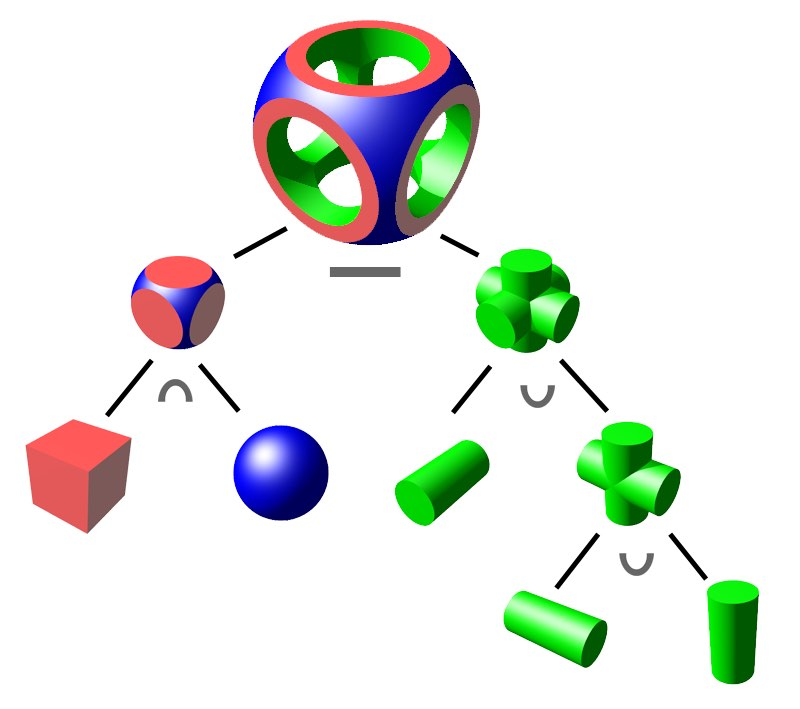
\includegraphics[width=0.7\linewidth]{figs/csg}
\caption{A CSG object represented as a tree of Boolean set operations on a sphere, a cube and three cylinders. From Wikimedia Commons.}%
\label{fig:csg}
\end{figure}

\begin{description}
\item[Primitive instancing] defines simple solids parametrically, such as a sphere based on a radius and the coordinates of its centre\marginnote{primitive instancing}\index{primitive instancing};
\item[Arbitrary polyhedra] defined using mesh data structures and boundary representation; and
\item[Half-spaces] (\reffig{halfspaces})\marginnote{half-space}\index{half-space} defined using a plane equation and a direction.
\end{description}

\begin{figure}
\centering
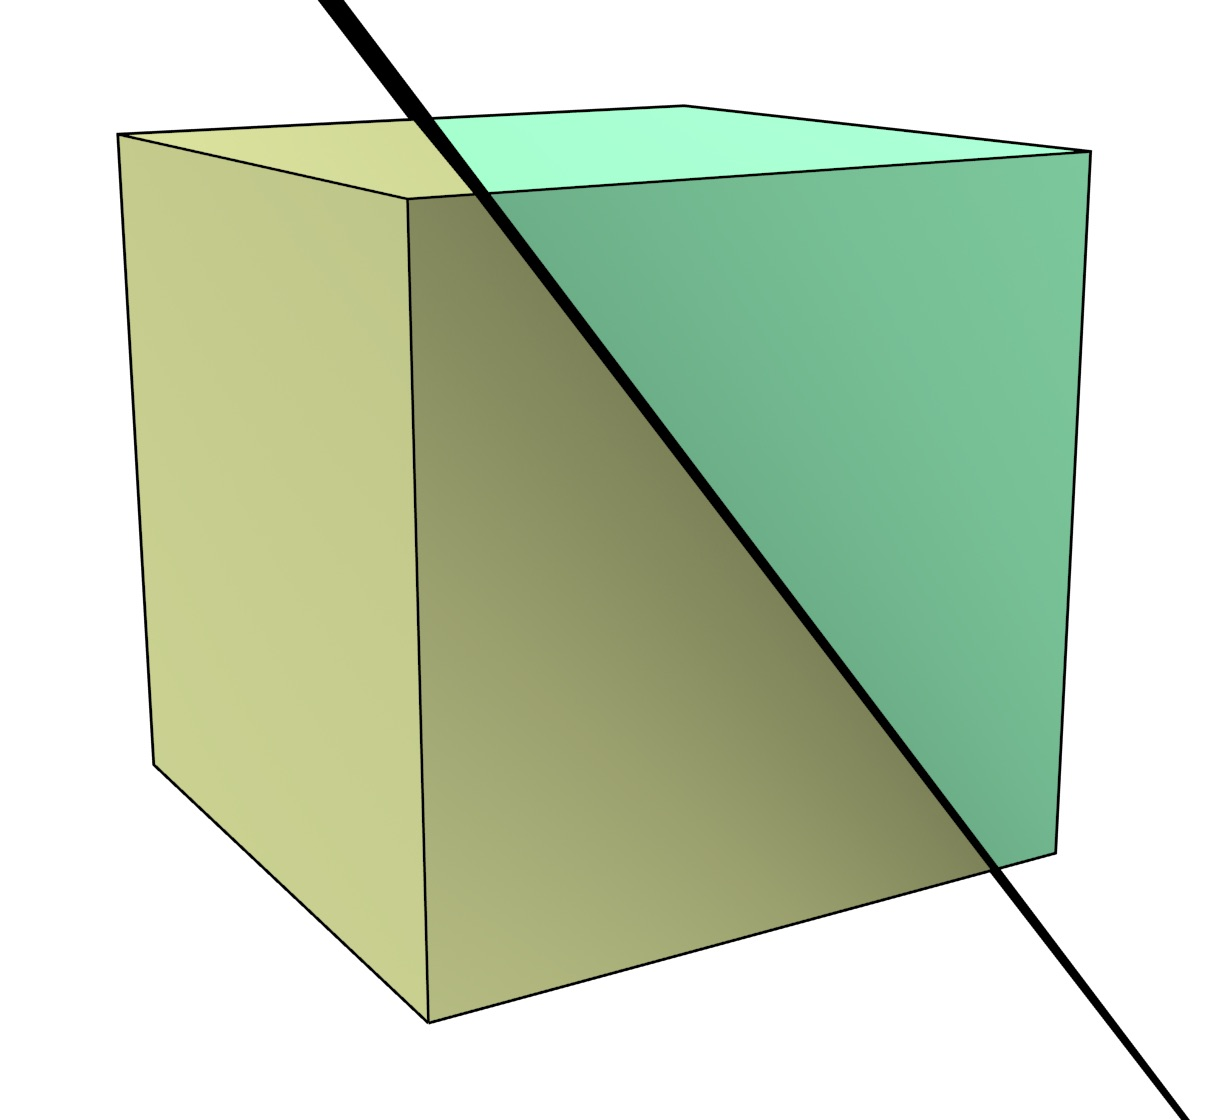
\includegraphics[width=0.3\linewidth]{figs/halfspaces}
\caption{A plane separates 3D space into two parts on either side of it. A plane and a direction can thus be used to specify the geometry of one of these halves, which forms an unbounded space on all directions except one.}%
\label{fig:halfspaces}
\end{figure}

The next section of the handout is a short summary of the mathematical background for this lesson, which consists of set theory, Boolean set operations and their mathematical notation.
Feel free to skip it if you are familiar with them.
In the next two sections, we look at how the two main elements of CSG work in theory: (i) the definition of simple objects as point sets, and (ii) how these elements can be combined using Boolean point set operations.
The final section covers Nef polyhedra, which are arguably the best known basis to implement CSG in practice.

\section{Background: set theory and Boolean set operations}

Set theory\marginnote{set theory}\index{set theory} is the branch of mathematics that studies \emph{sets}\marginnote{set}\index{set}, which are collections of abstract objects.
These objects can be anything, including other sets.

Set theory starts by considering the existence of a given domain of objects from which one may build sets, which is known as the \emph{universe set}\marginnote{universe set}\index{universe set} and denoted as \(\mathbb{U}\).
If an object \(a\) is part of a set \(\mathbb{X}\), it is denoted as \(a \in \mathbb{X}\), which is read as `\(a\) is an \emph{element}\marginnote{element of a set}\index{element of a set} of \(\mathbb{X}\)'.
If \(a\) is not part of a set \(\mathbb{X}\), it is denoted as \(a \notin \mathbb{X}\), which is read as `\(a\) is not an element of \(\mathbb{X}\)'.
By convention, lower case is usually used for simple elements and upper case for sets.

There are two common ways to describe the elements in a set, both using curly braces, \ie\ \{ and \}.
One way to do so is to list all the elements of the set one by one.
For instance, the set \(\left\{ 1,2,3 \right\}\) is the set containing \(1\), \(2\) and \(3\) as elements (and no others).
The other way to do so is to specify one or more rules that the elements of the set need to fulfil.
For instance, the set \(\{ x : x\)~\emph{is~a~prime~number}\(\}\) consists of all prime numbers.
It is read as `\(x\), such that \(x\) is a prime number'.

The order in which the elements in a set are defined does not matter.
That is, \(\left\{ 1,2,3 \right\}\) and \(\left\{ 3,2,1 \right\}\) are the same set.
The elements in a set are also unique, and duplicate items are ignored by convention.
That is, \(\left\{ 1,2,3 \right\}\) and \(\left\{ 1,2,3,2,1 \right\}\) are also the same set.

A set may contain an infinite number of elements (\eg\ as the prime number example above), or no elements at all, in which case it is a special set known as the \emph{null set}\marginnote{null set}\index{null set} or \emph{empty set}\marginnote{empty set}\index{empty set} and denoted as \(\{ \}\) or \(\emptyset\).
Other commonly used sets with a special notation and name are: the natural numbers (\(\mathbb{N}\)), the real numbers (\(\mathbb{R}\)), the rational numbers (\(\mathbb{Q}\)) and the integers (\(\mathbb{Z}\)).

In order to build more complex sets, the concepts and notation from mathematical logic are used, in particular \emph{propositional logic}\marginnote{propositional logic}\index{propositional logic}.
Propositional logic works with \emph{propositions}\marginnote{proposition}\index{proposition}, which are sentences that are either true or false, but not both.
These propositions might be altered and combined using various symbols expressing various notions, such as: \emph{and} (\(\wedge\)), \emph{or} (\(\vee\)), \emph{not} (\(\neg\)), \emph{implies} (\(\Rightarrow\)), \emph{is implied by} (\(\Leftarrow\)), \emph{if and only if} (\(\Leftrightarrow\)), \emph{for all} (\(\forall\)) and \emph{exists} (\(\exists\)).
These symbols correspond to their names.
For instance, \(a \wedge b\) is true only when both \(a\) and \(b\) are true, \(a \vee b\) is true when \(a\) or \(b\) are true (or both), and \(\neg a\) is true when \(a\) is false.

Using these concepts it is possible to state relationships between sets\marginnote{relationship between sets}\index{relationship between sets}.
For instance, we can define that \(\mathbb{A}\) and \(\mathbb{B}\) are equal (\(\mathbb{A} = \mathbb{B}\)) when an element is in \(\mathbb{A}\) if and only if it is also in \(\mathbb{B}\), which can be denoted as \(\forall x : x \in \mathbb{A} \Leftrightarrow x \in \mathbb{B}\).
A set \(\mathbb{A}\) is called a subset\marginnote{subset}\index{subset} of a set \(\mathbb{B}\) (\(\mathbb{A} \subseteq \mathbb{B}\)), or \(\mathbb{B}\) is a superset\marginnote{superset}\index{superset} of \(\mathbb{A}\) (\(\mathbb{B} \supseteq \mathbb{A}\)), when if an element is in \(\mathbb{A}\) then it is also in \(\mathbb{B}\), denoted as \(\forall x : x \in \mathbb{A} \Rightarrow x \in \mathbb{B}\).
If \(\mathbb{A} \subseteq \mathbb{B}\) but \(\mathbb{A} \neq \mathbb{B}\), \ie\ there is at least one extra element in \(\mathbb{B}\), then \(\mathbb{A}\) is a proper subset\marginnote{proper subset}\index{proper subset} of \(\mathbb{B}\) (\(\mathbb{A} \subset \mathbb{B}\)), or alternatively \(\mathbb{B}\) is a proper superset\marginnote{proper superset}\index{proper superset} of \(\mathbb{A}\) (\(\mathbb{B} \supset \mathbb{A}\)).
Note that these relationships are akin to `less than' (\(<\)), `less or equal than' (\(\leq\)), `equal to' (\(=\)), `greater or equal than' (\(\geq\)), and `greater than' (\(>\)) for numbers.

It is also possible to use propositional logic to create new sets by defining certain operations between sets, in particular \emph{Boolean set operations}\marginnote{Boolean set operation}\index{Boolean set operation}, consisting of intersection, union, difference and complement.
The intersection\marginnote{intersection}\index{intersection} of the sets \(\mathbb{A}\) and \(\mathbb{B}\), denoted as \(\mathbb{A} \cap \mathbb{B}\), consists of all the elements that are both in \(\mathbb{A}\) and in \(\mathbb{B}\), \ie\ \(\mathbb{A} \cap \mathbb{B} = \left\{ x : x \in \mathbb{A} \wedge x \in \mathbb{B} \right\}\).
The union\marginnote{union}\index{union} of the sets \(\mathbb{A}\) and \(\mathbb{B}\), denoted as \(\mathbb{A} \cup \mathbb{B}\), consists of all the elements that are either in \(\mathbb{A}\) or in \(\mathbb{B}\), \ie\ \(\mathbb{A} \cup \mathbb{B} = \left\{ x : x \in \mathbb{A} \vee x \in \mathbb{B} \right\}\).
The difference\marginnote{difference}\index{difference} between sets \(\mathbb{A}\) and \(\mathbb{B}\), denoted as \(\mathbb{A} - \mathbb{B}\), consists of all the elements that are in \(\mathbb{A}\) but not in \(\mathbb{B}\), \ie\ \(\mathbb{A} - \mathbb{B} = \left\{ x : x \in \mathbb{A} \wedge x \notin \mathbb{B} \right\}\).
The complement\marginnote{complement}\index{complement} of a set \(\mathbb{A}\), denoted as \(\neg \mathbb{A}\), consists of all the elements that are in the universe set but are not in \(\mathbb{A}\), \ie\ \(\neg \mathbb{A} = \left\{ x : x \in \mathbb{U} \wedge x \notin \mathbb{A} \right\}\).

Apart from sets, it is also possible to consider \emph{tuples}\marginnote{tuple}\index{tuple} of elements, which are sequences of ordered elements.
A tuple containing exactly two elements is known as a \emph{pair}\marginnote{pair}\index{pair}, one containing three elements is a \emph{treble}\marginnote{treble}\index{treble} and one containing \(n\) elements is an \(n\)-tuple.
Tuples are usually denoted using parenthesis, \ie\ (\ and~).

A common operation that generates tuples is the Cartesian product.
The Cartesian product\marginnote{Cartesian product}\index{Cartesian product} of sets \(\mathbb{A}\) and \(\mathbb{B}\), denoted as \(\mathbb{A} \times \mathbb{B}\), is defined as \(\left\{ (a,b) : a \in \mathbb{A} \wedge b \in \mathbb{B} \right\}\).
In other words, it is a set of pairs, where the first element of a pair is an element of \(\mathbb{A}\) and the second element of the pair is an element of \(\mathbb{B}\).
This can be generalised to more than two sets, such that the \(n\)-fold Cartesian product of \(n\) sets is an \(n\)-tuple.
The \(n\)-fold Cartesian product of a set \(\mathbb{A}\) with itself, \ie\ \(\mathbb{A} \times \mathbb{A} \times \cdots \mathbb{A}\), is denoted as \(\mathbb{A}^n\).

\section{Defining objects using point set geometry}%
\label{sec:ps}

Point set geometry applies the notions of set theory to define the geometry of objects as sets of points.
The usual definition maps 1D space (\ie\ the line) to the set of real numbers (\ie\ \(\mathbb{R}\)), and so 2D space (\ie\ the plane) is \(\mathbb{R}^2\) and 3D space is \(\mathbb{R}^3\).

Individual points in 2D and 3D space can be considered as elements of \(\mathbb{R}^2\) and \(\mathbb{R}^3\).
For instance, we can denote a point \(p\) in 2D space as \(p \in \mathbb{R}^2\) or in 3D space as \(p \in \mathbb{R}^3\).
Note that this notation perfectly matches the way in which points are usually defined based on their coordinates.
For example, by stating \(p = (x, y, z) \in \mathbb{R}^3\), we simply mean that \(x,y,z \in \mathbb{R} \), \ie\ that \(x\), \(y\) and \(z\) are arbitrary real numbers.

Based on these definitions, we can then define sets that describe specific geometric objects.
For instance, we can start by considering how any point \(p\) between two points \(p_1\) and \(p_2\) at different locations can be obtained as a sort of weighted average of \(p_1\) and \(p_2\), where the relative weight of the two points tell us that we're closer to one point than to another.
If we put this into an equation, we get:

\begin{equation}
p = \frac{a p_1 + b p_2}{a+b}.
\end{equation}

Note that we divide everything by \(a+b\) to make sure that the weights add up to one.
Also, note it is possible to use negative weights to get points that are on the line that passes through \(a\) and \(b\) but not between \(a\) and \(b\).
Expanding on this, the line \(L\)\marginnote{point set equation of a line}\index{point set equation of a line} passing through \(p_1\) and \(p_2\) is defined by considering all possible values of \(a\) and \(b\).
That is:

\begin{equation}
\label{eq:line}
L = \left\{ \frac{a p_1 + b p_2}{a+b} : a,b \in \mathbb{R} \right\}.
\end{equation}

In the case of a line, we can get rid of one parameter by substituting \(t = a/(a+b)\), which would yield \(L = \left\{ t p_1 + (1-t) p_2 : t \in \mathbb{R} \right\} \).
Note how at \(t = 0\) we get \(p_2\), at \(t = 1\) we get \(p_1\), and when \(0 < t < 1\) we get the line segment between \(p_1\) and \(p_2\).
Note also how this definition of a line works both in 2D and 3D.

Generalising from \refeq{line}, we can also define a similar equation for a plane \(P\)\marginnote{point set equation of a plane}\index{point set equation of a plane} from three non-collinear points \(p_1\), \(p_2\) and \(p_3\) as:

\begin{equation}
P = \left\{ \frac{a p_1 + b p_2 + c p_3}{a+b+c} : a,b,c \in \mathbb{R} \right\}.
\end{equation}

In 3D, if we substitute the equality (\(=\)) of the previous equation for a strict inequality (\(<\) or \(>\)), we get instead an equation to represent the half-spaces\marginnote{point set equation of a half-space}\index{point set equation of a half-space} respectively below and above the plane (such as those previously shown in \reffig{halfspaces}).
An equation of this form is typically stored in the leaves of a CSG tree, \eg\ as the three non-collinear points in the equation above, or as the coefficients of an equation of the form \(ax + by + cz + d = 0 \), plus a direction to specify which half-space to use.

For the sake of uniformity and ease of processing, many CSG implementations only use half-spaces.
However, several simple axis-aligned 3D solids also have easy point set definitions that can be used to store them as primitives based on a few parameters, including:

\begin{description}
\item[balls] \ie\ the space inside a sphere\marginnote{point set equation of a ball}\index{point set equation of a ball}, which can be defined as \( (x-c_x)^2 + (y-c_y)^2 + (z-c_z)^2 < r^2\), where \(r\) is the radius and \(c = (c_x, c_y, c_z)\) is the centre;
\item[ellipsoid interiors] defined\marginnote{point set equation of an ellipsoid}\index{point set equation of an ellipsoid} as \( \frac{(x-c_x)^2}{a^2} + \frac{(y-c_y)^2}{b^2} + \frac{(z-c_z)^2}{c^2} < 1 \), where \(a\), \(b\) and \(c\) are half the lengths of each axis, and \(c = (c_x, c_y, c_z)\) is the centre; and
\item[cuboid interiors] \ie\ box-shaped objects\marginnote{point set equation of a cuboid}\index{point set equation of a cuboid}, which can be defined using intervals for the minimum and maximum values it has along each axis, \ie\ \( x_\mathrm{min} < x < x_\mathrm{max} \wedge y_\mathrm{min} < y < y_\mathrm{max} \wedge z_\mathrm{min} < z < z_\mathrm{max} \); and
\item[cylinder interiors] by\marginnote{point set equation of a cylinder}\index{point set equation of a cylinder} checking whether a point lies within a radius for two axes, and within an interval for the third.
\end{description}

Other common objects are more general versions of these objects, such as parallelepipeds, (truncated) cones, etc.
As for non-axis aligned simple solids, they can be supported by special nodes in the CSG tree that represent geometric transformations by their parameters (rather than Boolean point set operations), such as translations, rotations and scaling, or more general ones like affine transformations or arbitrary transformation matrices by storing their elements one by one.

\section{Boolean point set operations}
\label{sec:psetops}

In order to create objects other than those directly added to an implementation (\ie\ half-spaces and possibly some geometric shapes), CSG relies on Boolean point set operations (\reffig{boolean}).
Arbitrary polyhedra can be represented in this way by first splitting them into convex parts\marginnote{convex decomposition}\index{convex decomposition} (which might require Steiner vertices), and then representing the convex parts as intersections of half-spaces (one per face).
These operations, which are located in the non-leaf nodes of the CSG tree, combine the geometry of the point sets described by their children (using the methods described in the previous section).

\begin{figure}
\centering
\begin{subfigure}[b]{0.5\linewidth}
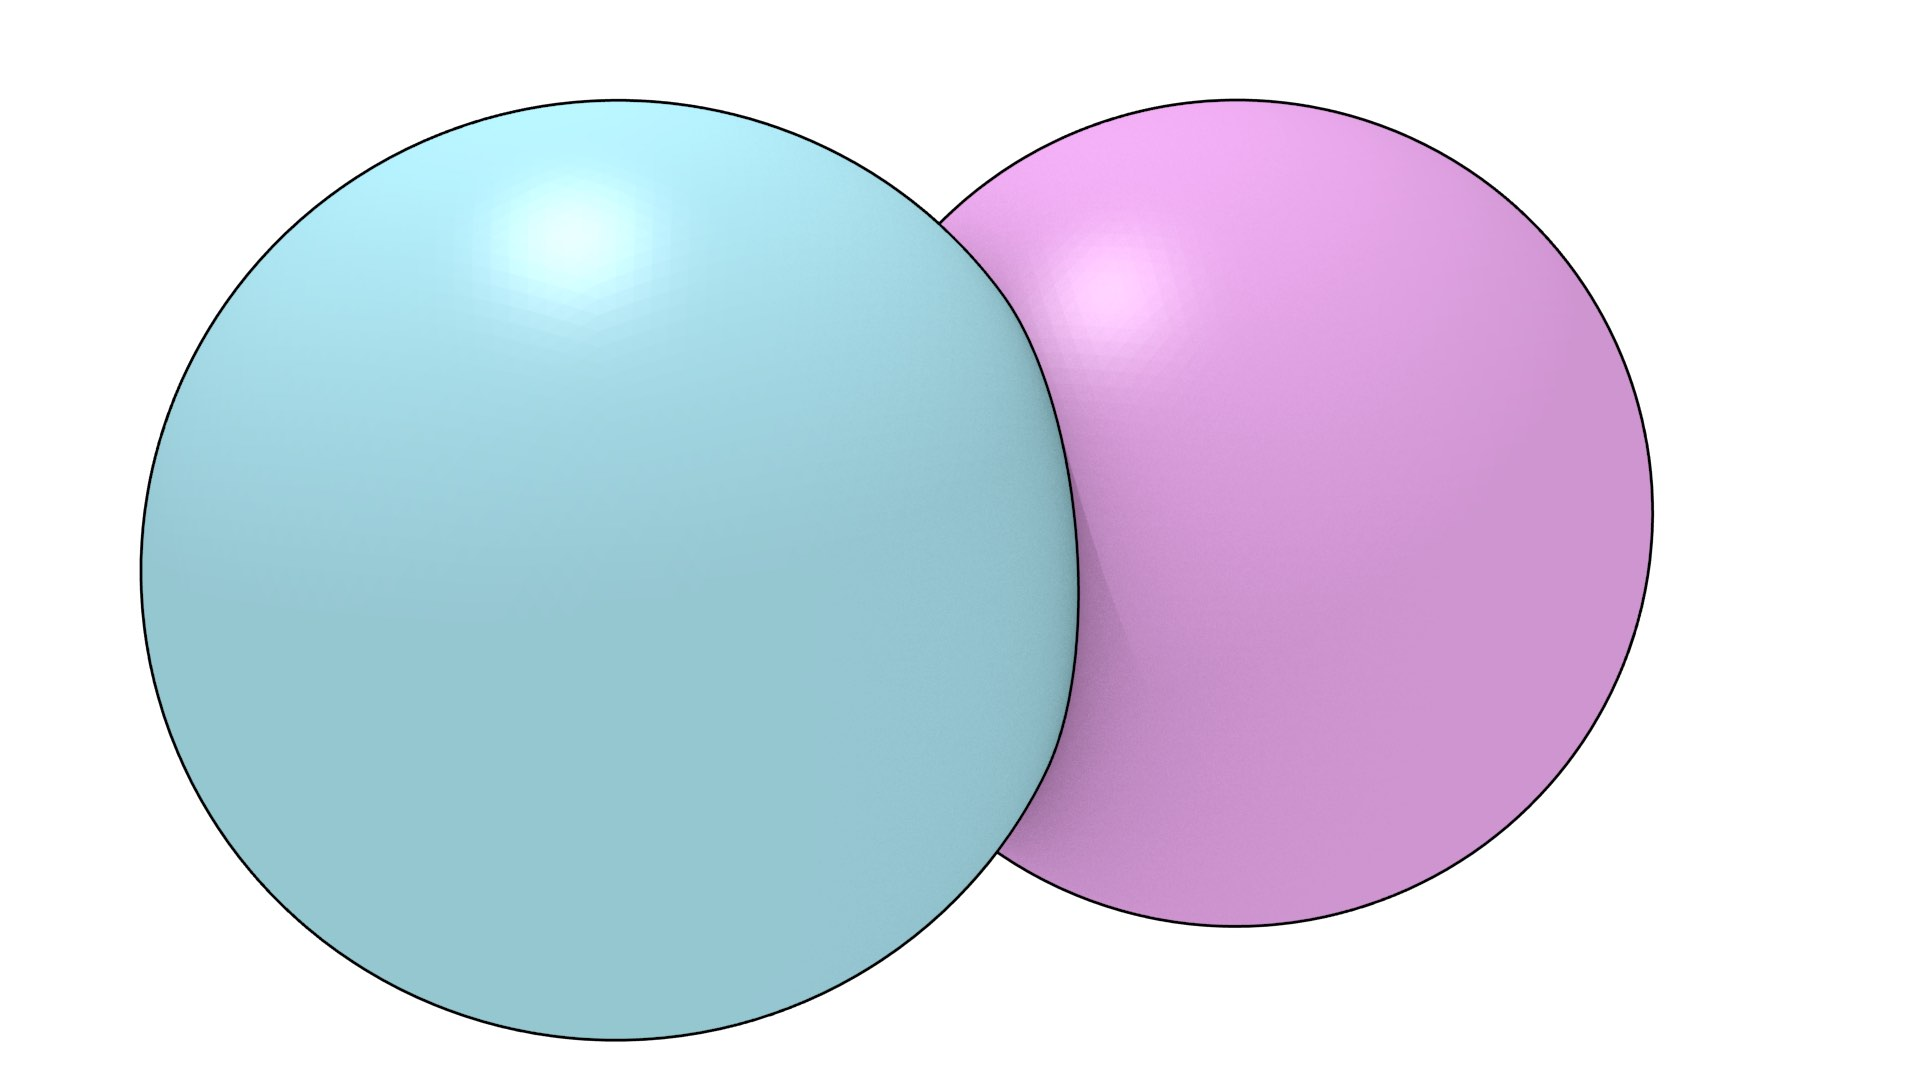
\includegraphics[width=\linewidth]{figs/boolean}
\caption{}%
\label{subfig:boolean}
\end{subfigure}%
\begin{subfigure}[b]{0.5\linewidth}
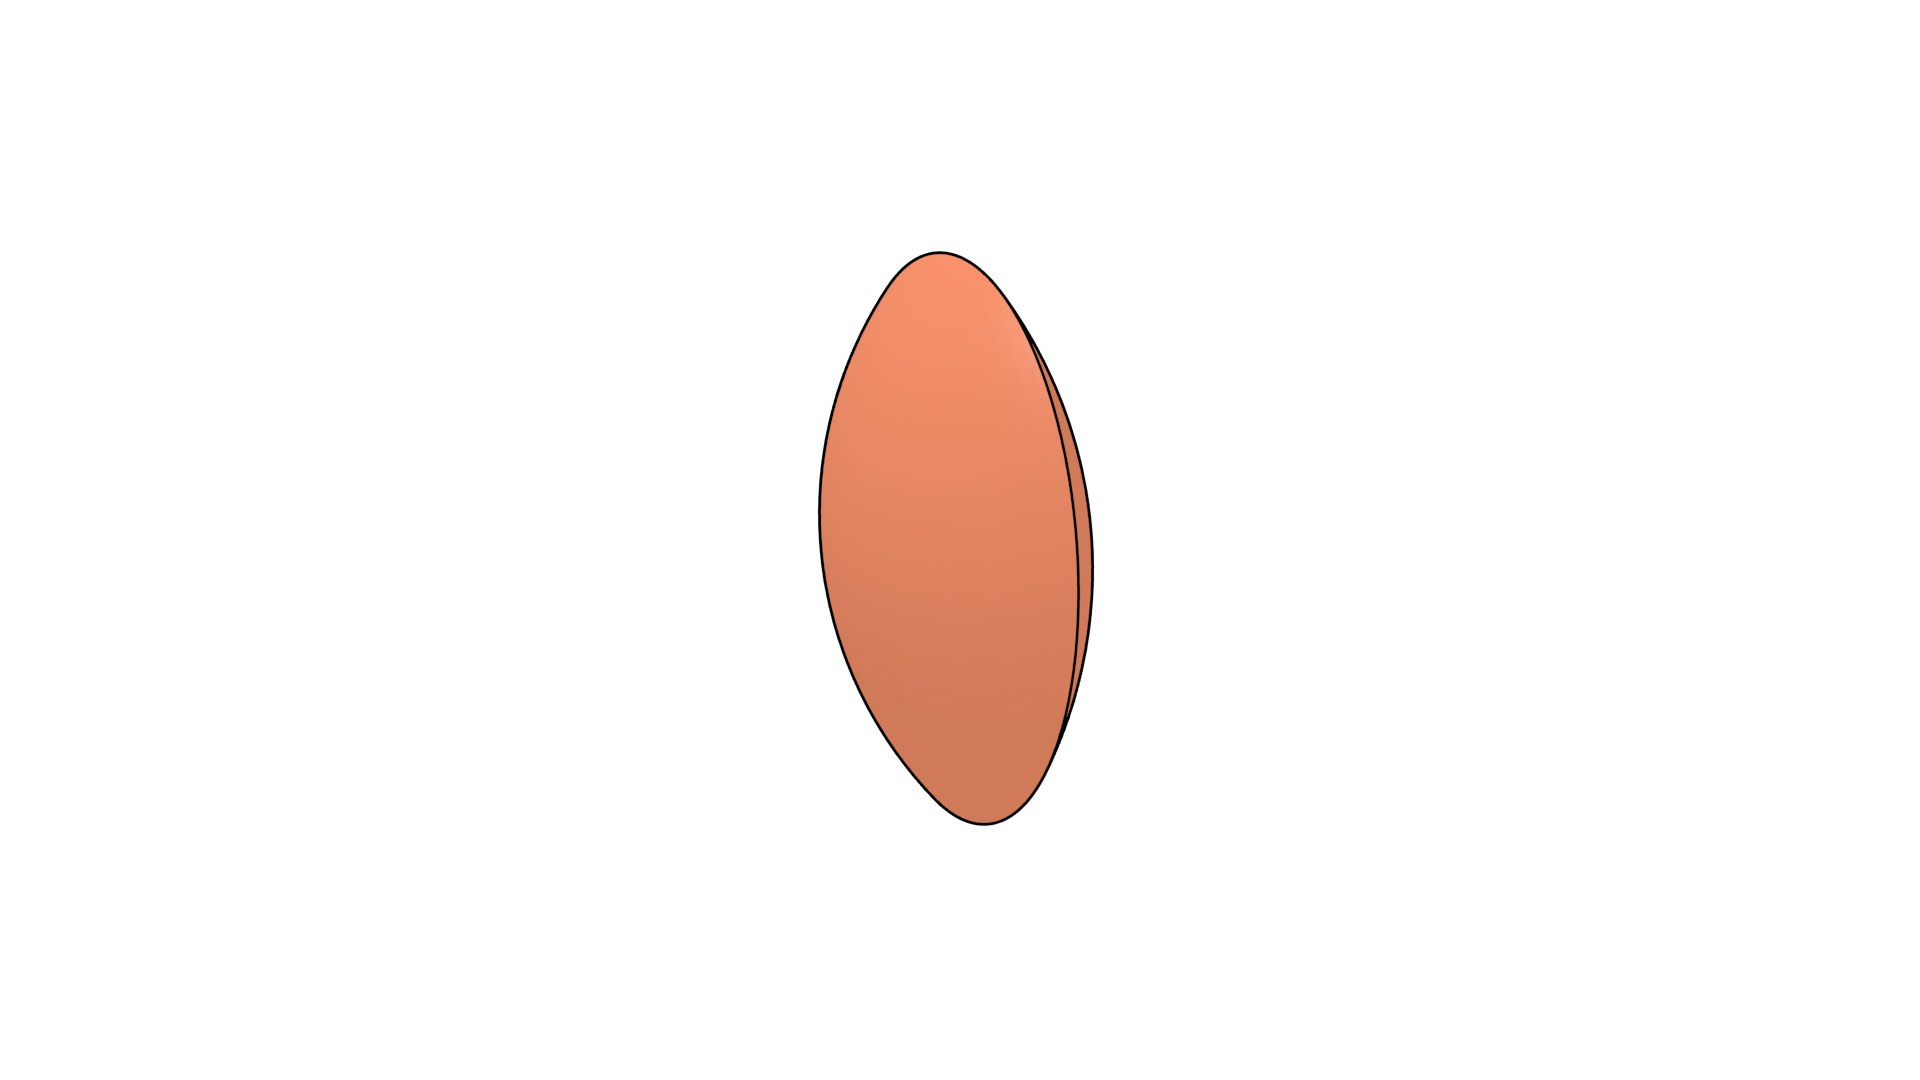
\includegraphics[width=\linewidth]{figs/boolean-intersection}
\caption{}%
\label{subfig:boolean-intersection}
\end{subfigure}\\
\begin{subfigure}[b]{0.5\linewidth}
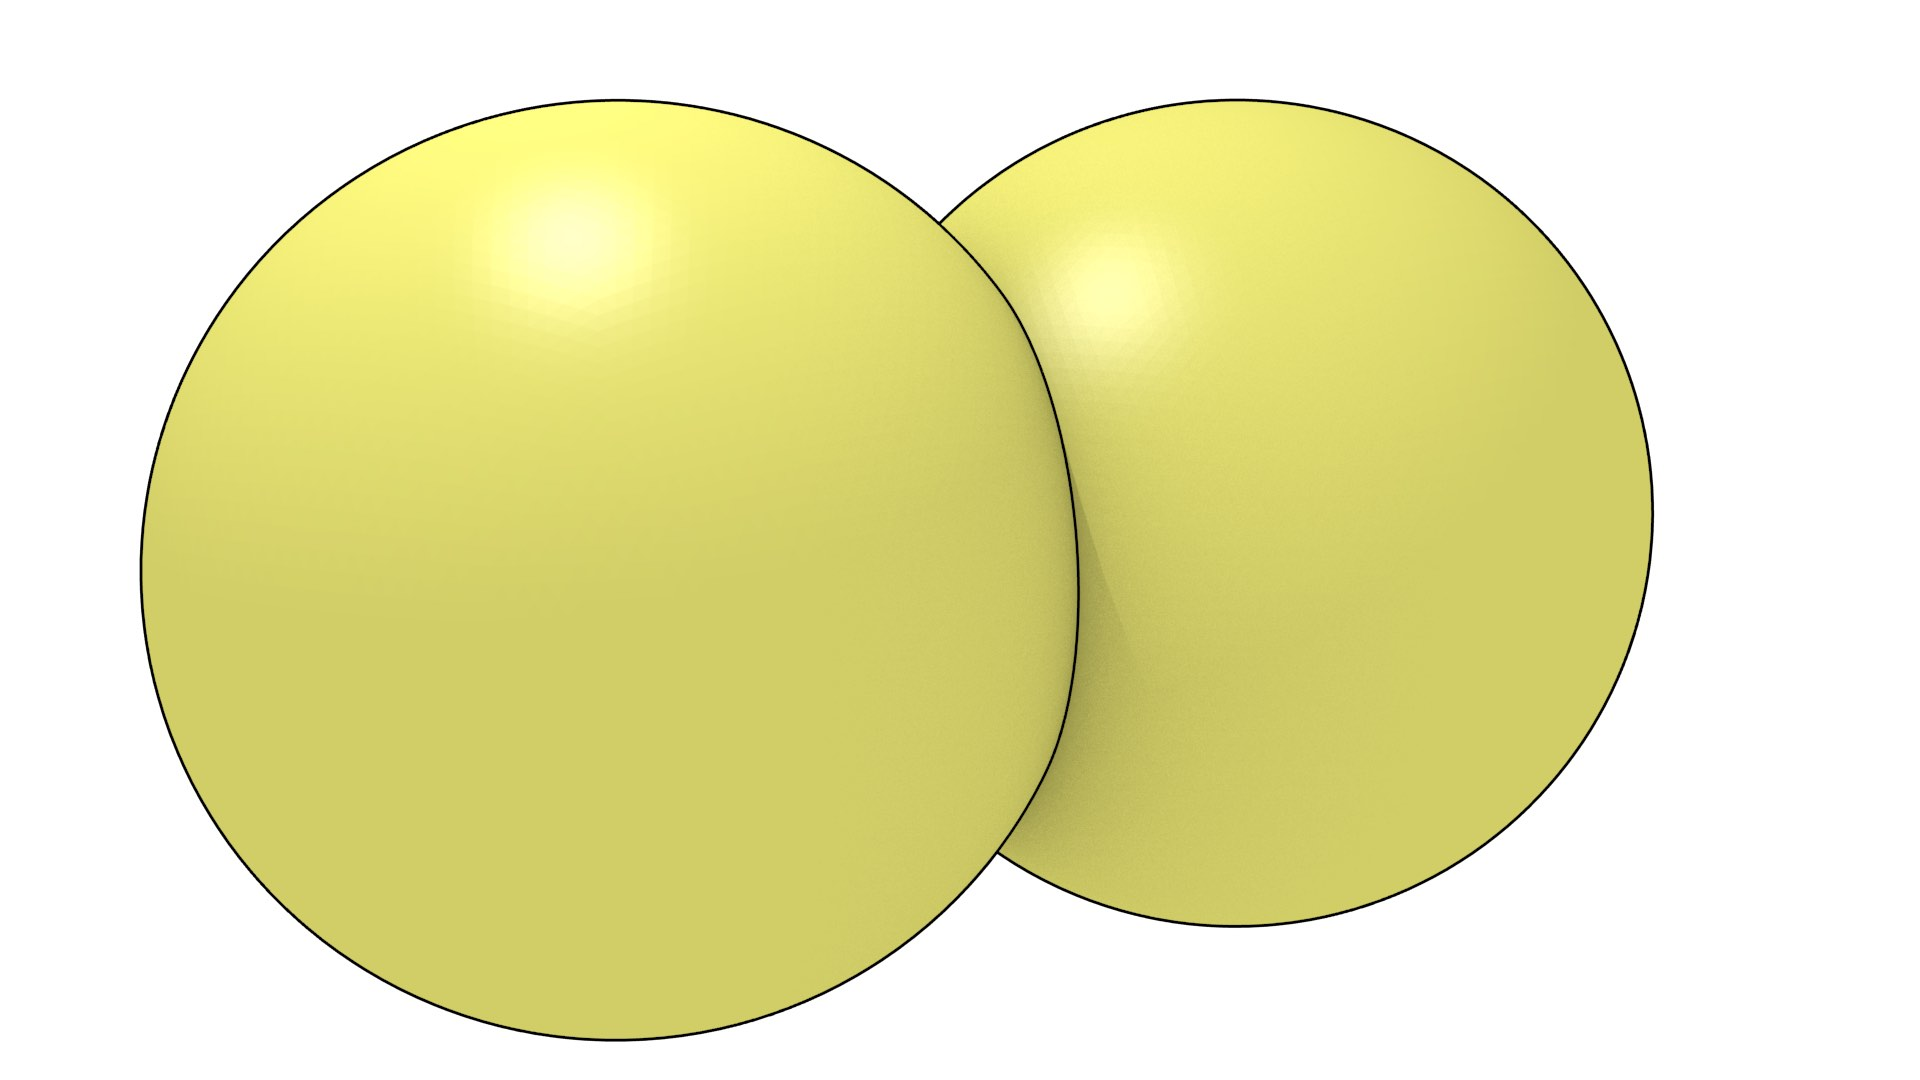
\includegraphics[width=\linewidth]{figs/boolean-union}
\caption{}%
\label{subfig:boolean-union}
\end{subfigure}%
\begin{subfigure}[b]{0.5\linewidth}
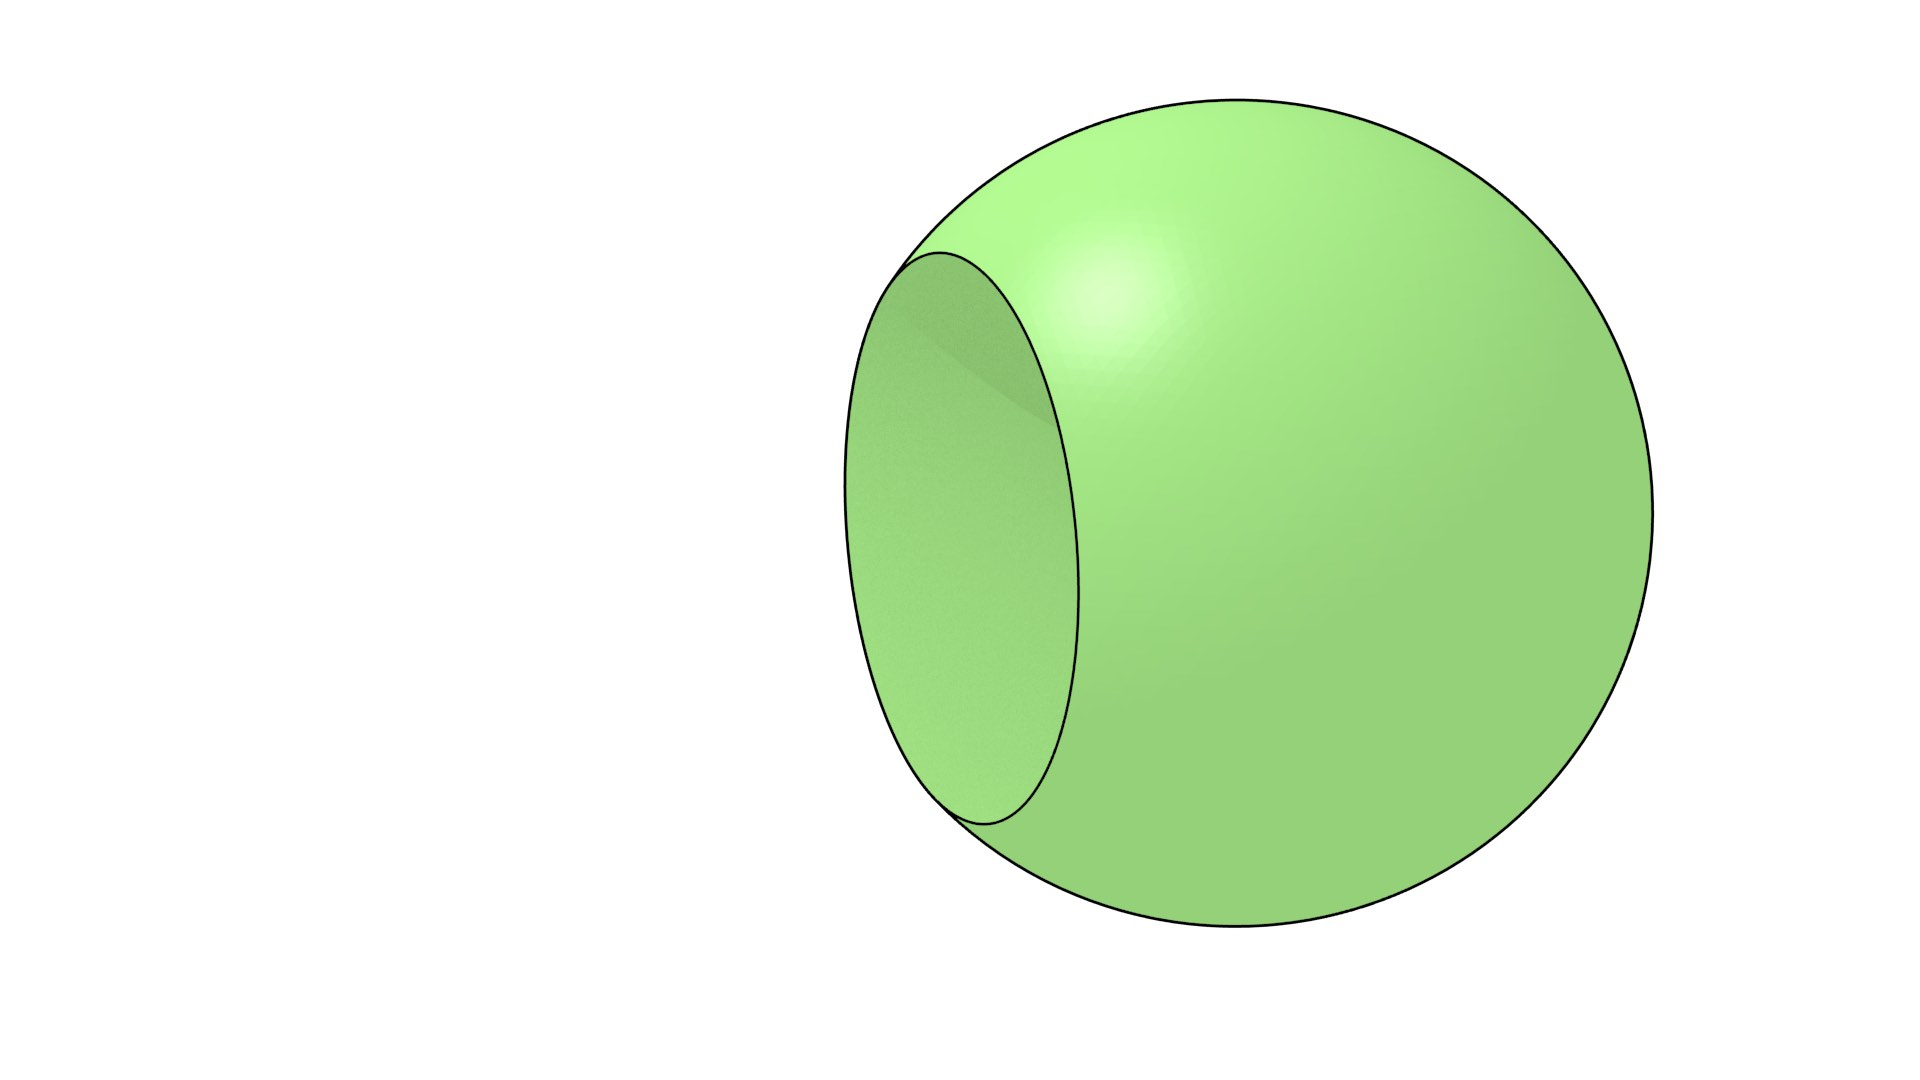
\includegraphics[width=\linewidth]{figs/boolean-difference}
\caption{}%
\label{subfig:boolean-difference}
\end{subfigure}
\caption{Based on (a) two balls \(\mathbb{A}\) and \(\mathbb{B}\), other objects can be defined using Boolean set operations, such as: (b) the intersection \(\mathbb{A} \cap \mathbb{B}\), (c) the union \(\mathbb{A} \cup \mathbb{B}\), and (d) the difference \(\mathbb{A} - \mathbb{B}\).}%
\label{fig:boolean}
\end{figure}

Boolean point set operations are based on the Boolean operations on sets, which are mainly:

\begin{description}
\item[union] of\marginnote{union}\index{union} the sets \(\mathbb{A}\) and \(\mathbb{B}\), denoted as \(\mathbb{A} \cup \mathbb{B}\), is the set containing the elements that are in \(\mathbb{A}\) or \(\mathbb{B}\), \ie\ \( \mathbb{A} \cup \mathbb{B} = \left\{ x : x \in \mathbb{A} \vee x \in \mathbb{B} \right\} \);
\item[intersection] of\marginnote{intersection}\index{intersection} the sets \(\mathbb{A}\) and \(\mathbb{B}\), denoted as \(\mathbb{A} \cap \mathbb{B}\), is the set containing the elements that are in both \(\mathbb{A}\) and \(\mathbb{B}\), \ie\ \( \mathbb{A} \cap \mathbb{B} = \left\{ x : x \in \mathbb{A} \wedge x \in \mathbb{B} \right\} \);
\item[set difference] of\marginnote{difference}\index{difference} the sets \(\mathbb{A}\) and \(\mathbb{B}\), denoted as \(\mathbb{A} - \mathbb{B}\) or \(\mathbb{A} \setminus \mathbb{B}\), is the set containing the elements that are in \(\mathbb{A}\) but not in \(\mathbb{B}\), \ie\ \( \mathbb{A} - \mathbb{B} = \left\{ x : x \in \mathbb{A} \wedge x \notin \mathbb{B} \right\} \);
\item[symmetric difference] of\marginnote{symmetric difference}\index{symmetric difference} the sets \(\mathbb{A}\) and \(\mathbb{B}\), denoted as \(\mathbb{A} \triangle \mathbb{B}\), \(\mathbb{A} \ominus \mathbb{B}\) or \(\mathbb{A} \oplus \mathbb{B}\), is the set containing the elements that are either in \(\mathbb{A}\) or in \(\mathbb{B}\) but not in both, \ie\ \( \mathbb{A} \triangle \mathbb{B} = \left\{ x : x \in \mathbb{A} - \mathbb{B} \cup \mathbb{B} - \mathbb{A} \right\} \).
\end{description}

The key point about these operations is that they do not need to perform any geometric computations, since it is possible to tell if an element (\ie\ point) is in the new point set by just checking whether it is in its children's point sets.
It is thus trivially easy to do Boolean point set operations on individual points.

Based on this knowledge, we could build a crude CSG implementation directly on a point cloud or voxel grid by: (i) for each leaf node, checking whether each point/voxel meets the point set definition in the node, and (ii) for each non-leaf node, applying the Boolean set operations on the point sets represented by its child nodes point by point.
However, since this easy solution is not applicable to other data models, we will look at a better solution that works better in practice.

\section{Nef polyhedra}

\emph{Nef polyhedra}\marginnote{Nef polyhedra}\index{Nef polyhedra}, named after Walter Nef, are an alternative representation of polygons and polyhedra (\ie\ not the usual b-rep meshes) that is based on the concept of a \emph{local pyramid}, which is a structure that stores the neighbourhood information around every vertex (\reffig{nef}).
Polygons and polyhedra can be stored as a set of local pyramids and their location (as a set of 2D/3D coordinates).

\begin{figure}
\centering
\begin{subfigure}[b]{0.5\linewidth}
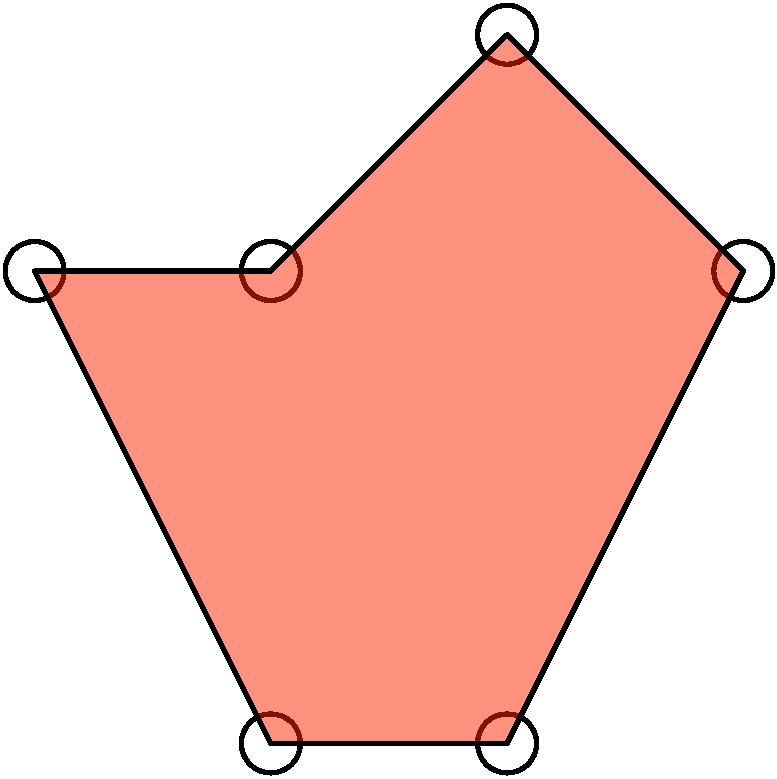
\includegraphics[width=\linewidth]{figs/nef-1}
\caption{}%
\end{subfigure}
\begin{subfigure}[b]{0.35\linewidth}
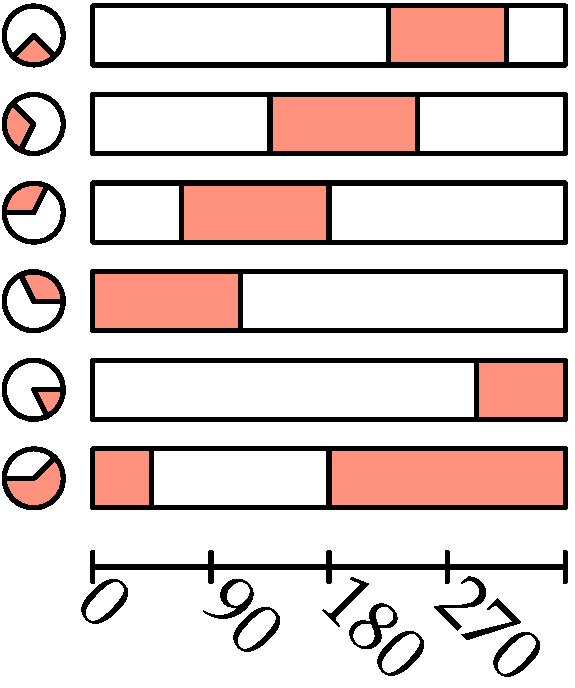
\includegraphics[width=\linewidth]{figs/nef-2}
\caption{}%
\end{subfigure}
\caption{(a) A Nef polygon is represented indirectly as (b) a set of local pyramids (circles).
At every local pyramid, the polygon (red) becomes an angular interval.
Incident edges become points at the endpoints of these intervals.}%
\label{fig:nef}
\end{figure}

\subsection{Local pyramids}

The local pyramid\marginnote{local pyramid}\index{local pyramid} of a vertex contains the intersection of an infinitesimally small sphere (in 3D) or circle (in 2D) with the volumes, faces and edges incident to this vertex.
An incident volume thus becomes a face, an incident face becomes an edge, and an incident edge becomes a vertex on the surface of the local pyramid sphere/circle, essentially lowering the dimension of every object by one (just like boundary representation does!).

The key thing to understand here is the following: \emph{a 2D/3D object represented as a set of local pyramids (and their location) can individually be stored using 1D/2D data structures}.
This is a process akin to boundary representation, but it does not have problems with non-manifold objects (unlike boundary representation).

In practice, computing the local pyramid at a local vertex is also a relatively simple operation.
We will not go through the details here (see the references in the notes if you are interested), but in 2D, it involves computing the angle of its neighbouring vertices as you rotate around the vertex, and marking the intervals between these vertices with the polygons that you pass through while doing so.
In 3D, it is a more complex operation involving the computation of an arrangement of lines in a spherical coordinate system, and the location of every neighbouring vertex is defined by two angles (rather than one).

\subsection{Computing Boolean point set operations on Nef polyhedra}

Boolean point set operations on Nef polyhedra (and many other geometric operations) can be computed in three steps: subdivision, selection and simplification.
This is a common scheme used in geometric computing in general, and we will discuss what each of these involves in this specific case.

\begin{description}

\item[Subdivision] involves\marginnote{subdivision}\index{subdivision} computing an overlay of the input polyhedra, thus creating the overall structure where the result will be put (\ie\ the vertices, edges, faces and volumes).

In 2D, this is also a computation of a line arrangement (also known in GIS as map overlay), where the output is a set of vertices and edges representing all the input lines of both polygons, but where edges do not intersect except at their common vertex end points.
Vertices (\ie\ local pyramids) will be located at the position of all input vertices and at every new intersection between lines.

In 3D, it is a similar operation, but the new vertices (\ie\ local pyramids) are located at line-polygon intersections as well.
These can be calculated by computing a plane passing through the polygon and intersecting it with the line.

\item[Selection] involves\marginnote{selection}\index{selection} checking whether each face (in 2D) or volume (3D) should be part of the output or not, marking it as such in the relevant parts of the local pyramids.
This is done by testing whether it is in the interior or exterior of the input Nef polygons/polyhedra.

\item[Simplification] involves\marginnote{simplification}\index{simplification} removing unnecessary structures in a way that does not alter the point set that is represented, which is akin to the dissolving operations common in GIS\@.
This is done by deleting local pyramids when they do not actually represent a new vertex, or when are not subdivided.

\end{description}

\reffig{nef-boolean} shows an example of how this works in practice in 2D.
A 2D Boolean point set operation starts from two Nef polygons \(A = (g, b, f, i)\) and \(B = (a, f, k, j, e, c)\)---each of which is stored as a set of local pyramids at its corresponding vertices.
As shown previously in \reffig{nef}, each of these 2D local pyramids can be stored as a list of 1D intervals, \eg\ at vertex \(a\), polygon \(B = [225, 315]\), where the values are in degrees.

The operation first computes the intersections between the line segments (as an overlay problem), creating the new vertices \(d\) and \(h\).
The location of these vertices can be calculated using the equations of the corresponding lines.
The vertices of each polygon and the intersection points between the line segments yield the local pyramids to be considered.

Then, the local pyramid intervals for both polygons at all of these locations are computed.
For instance, at vertex \(a\), \(A = \emptyset{}\) and \(B = [225, 315]\).
A Boolean set operation is then computed by applying it to the local pyramids (\ie\ to the intervals).
For instance, at vertex \(a\), \(\neg A = \mathbb{U} = [0, 360]\) and \(\neg B = [315, 225]\) (by inverting the range), \(A \cup B = [225, 315]\) (by combining the ranges), \(A \cap B = \emptyset{}\) (by finding common parts of the ranges), and \(A - B = \emptyset{}\) (by removing from the ranges of \(A\) those of \(B\)).

Finally, unnecessary local pyramids can be removed from the output: \(f\) in \(A \cup B\); \(a\), \(b\), \(c\), \(g\), \(i\), \(j\) and \(k\) in \(A \cap B\); and \(a\), \(c\), \(j\) and \(k\) in \(A - B\).

\begin{figure}
\centering
\begin{subfigure}[b]{0.23\linewidth}
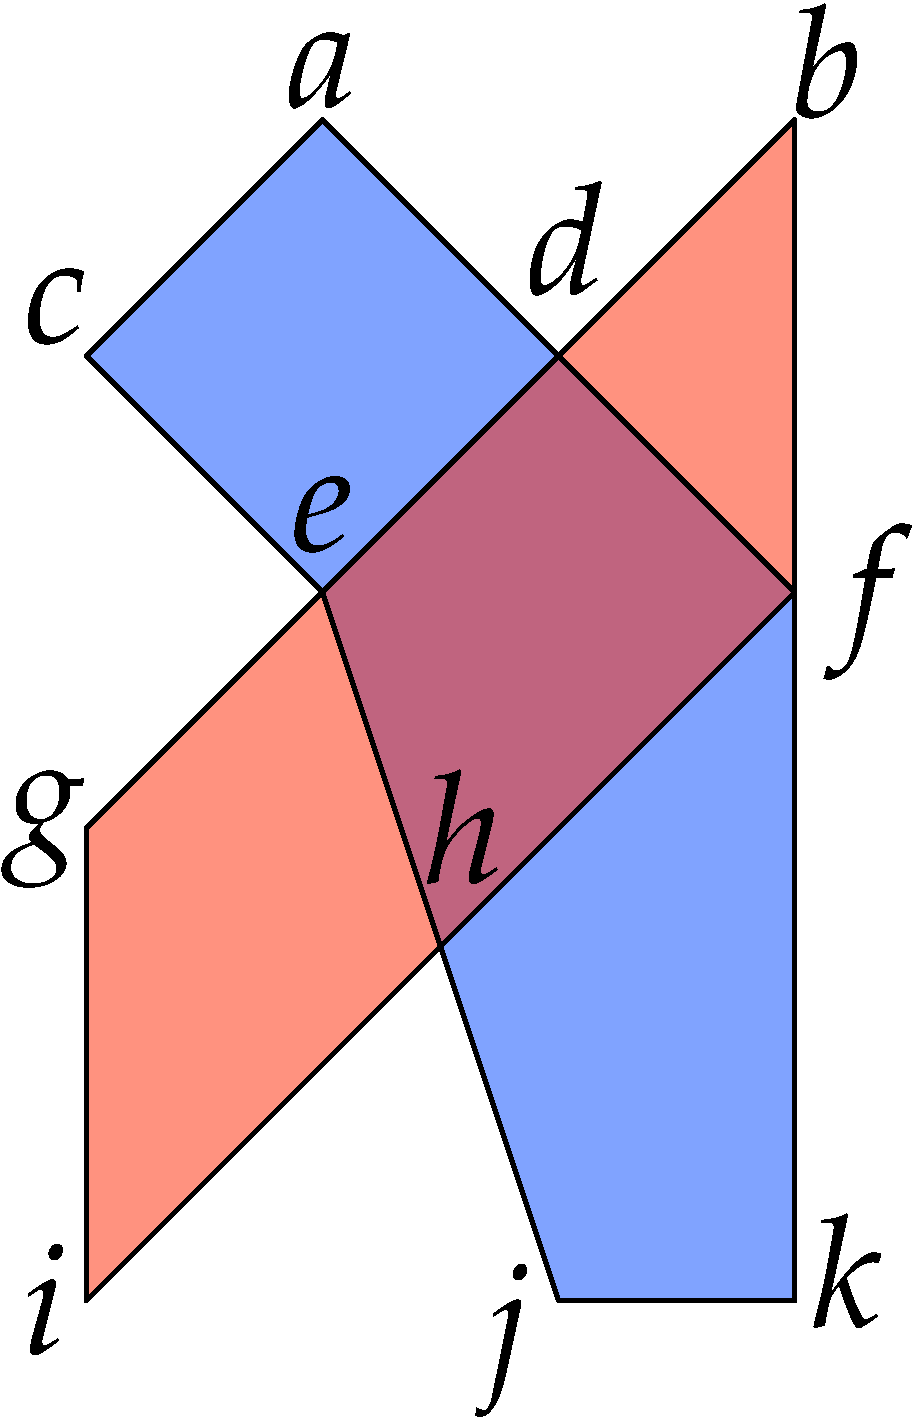
\includegraphics[width=\linewidth]{figs/nef-boolean-1}
\caption{}%
\end{subfigure}
\quad
\begin{subfigure}[b]{0.6\linewidth}
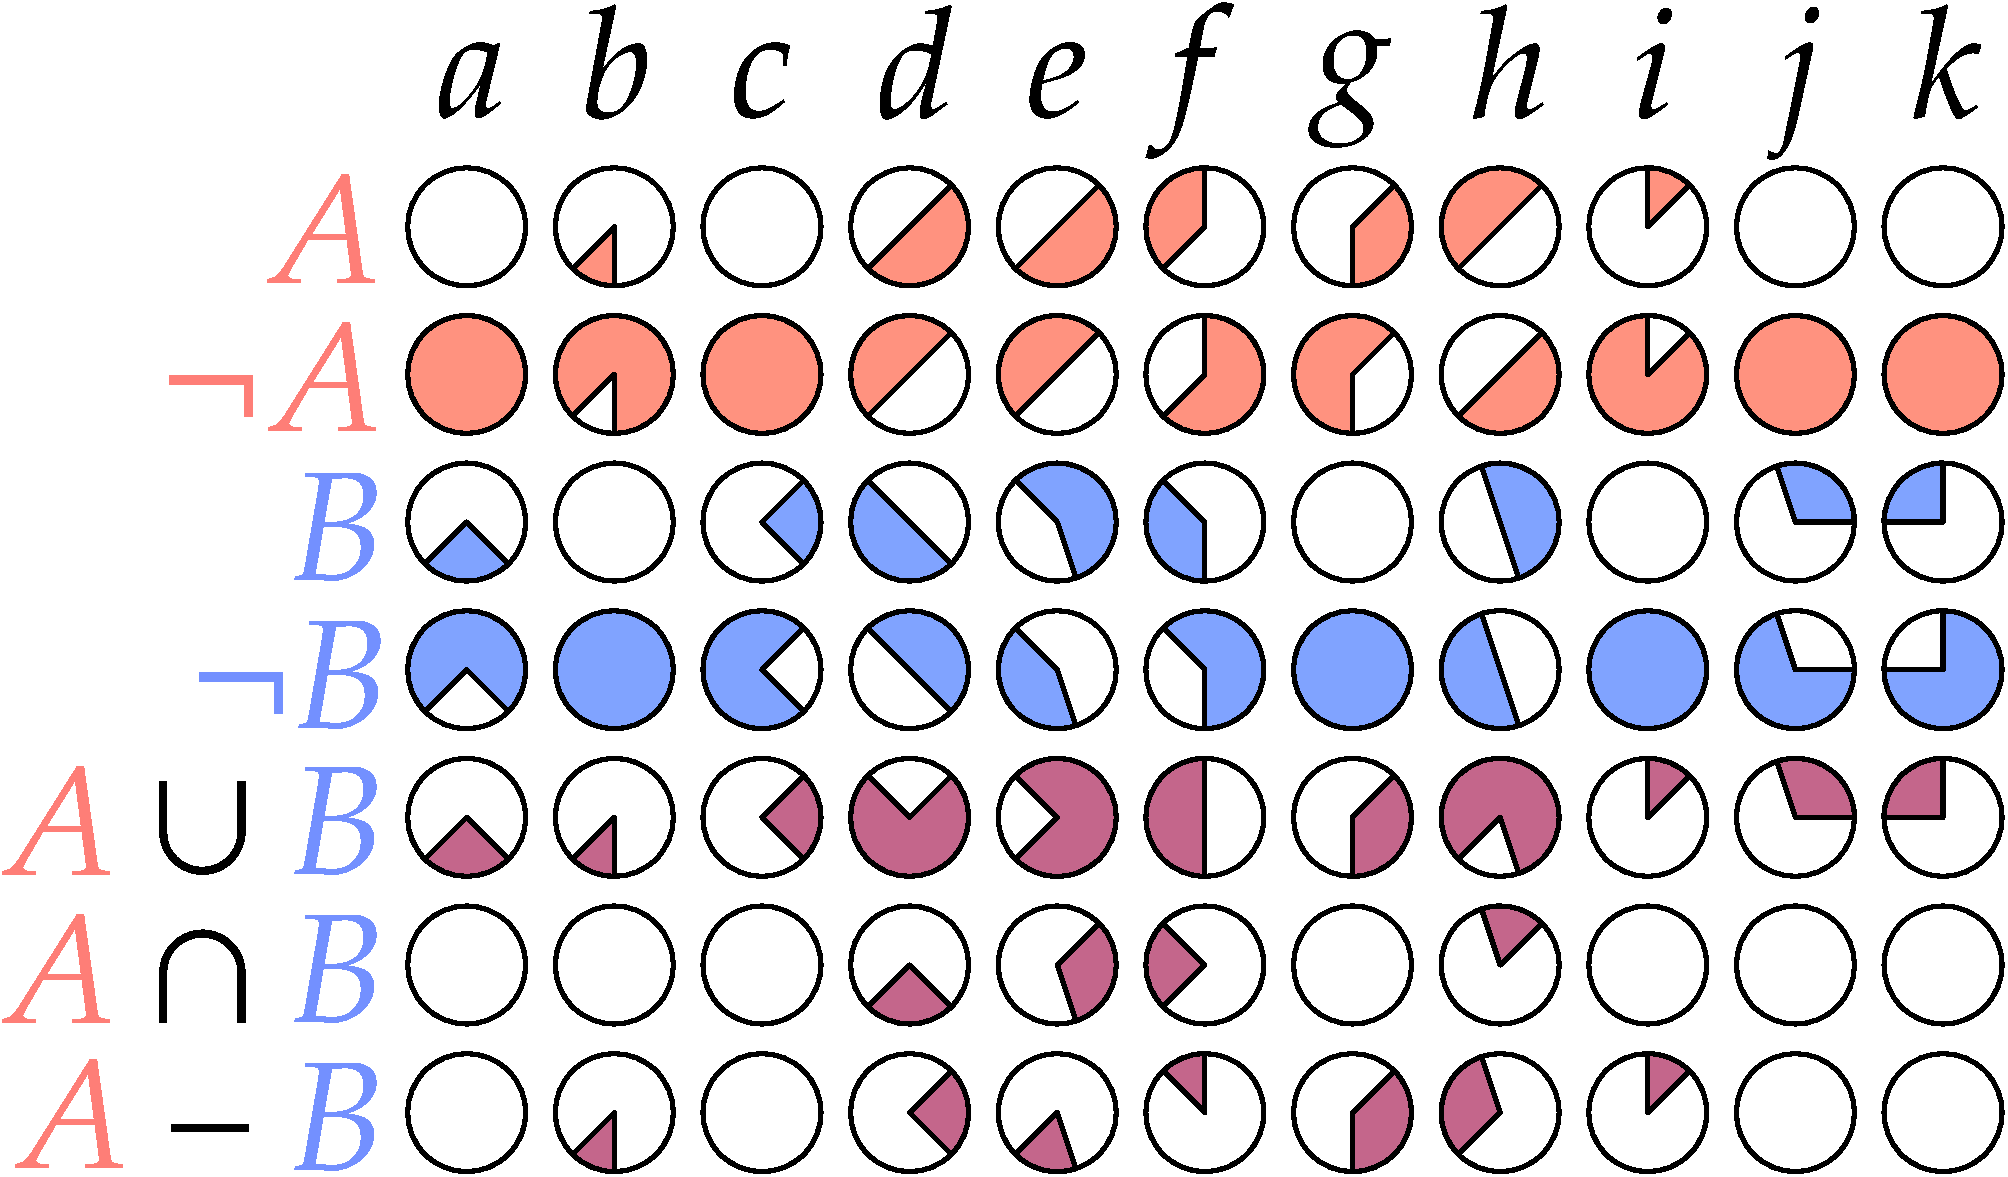
\includegraphics[width=\linewidth]{figs/nef-boolean-2}
\caption{}%
\end{subfigure}
\caption{Various Boolean point set operations on (a) the Nef polygons \(A\) (red) and \(B\) (blue) that can be performed on (b) their local pyramids.}%
\label{fig:nef-boolean}
\end{figure}

\subsection{3D Nef polyhedra in practice: selective Nef complexes}

3D Nef polyhedra and Boolean point set operations on them can be implemented using different data structures, but an excellent open implementation (see notes) uses a data structure called \emph{selective Nef complexes}\marginnote{selective Nef complex}\index{selective Nef complex} (\reffig{snc}).

\begin{figure}
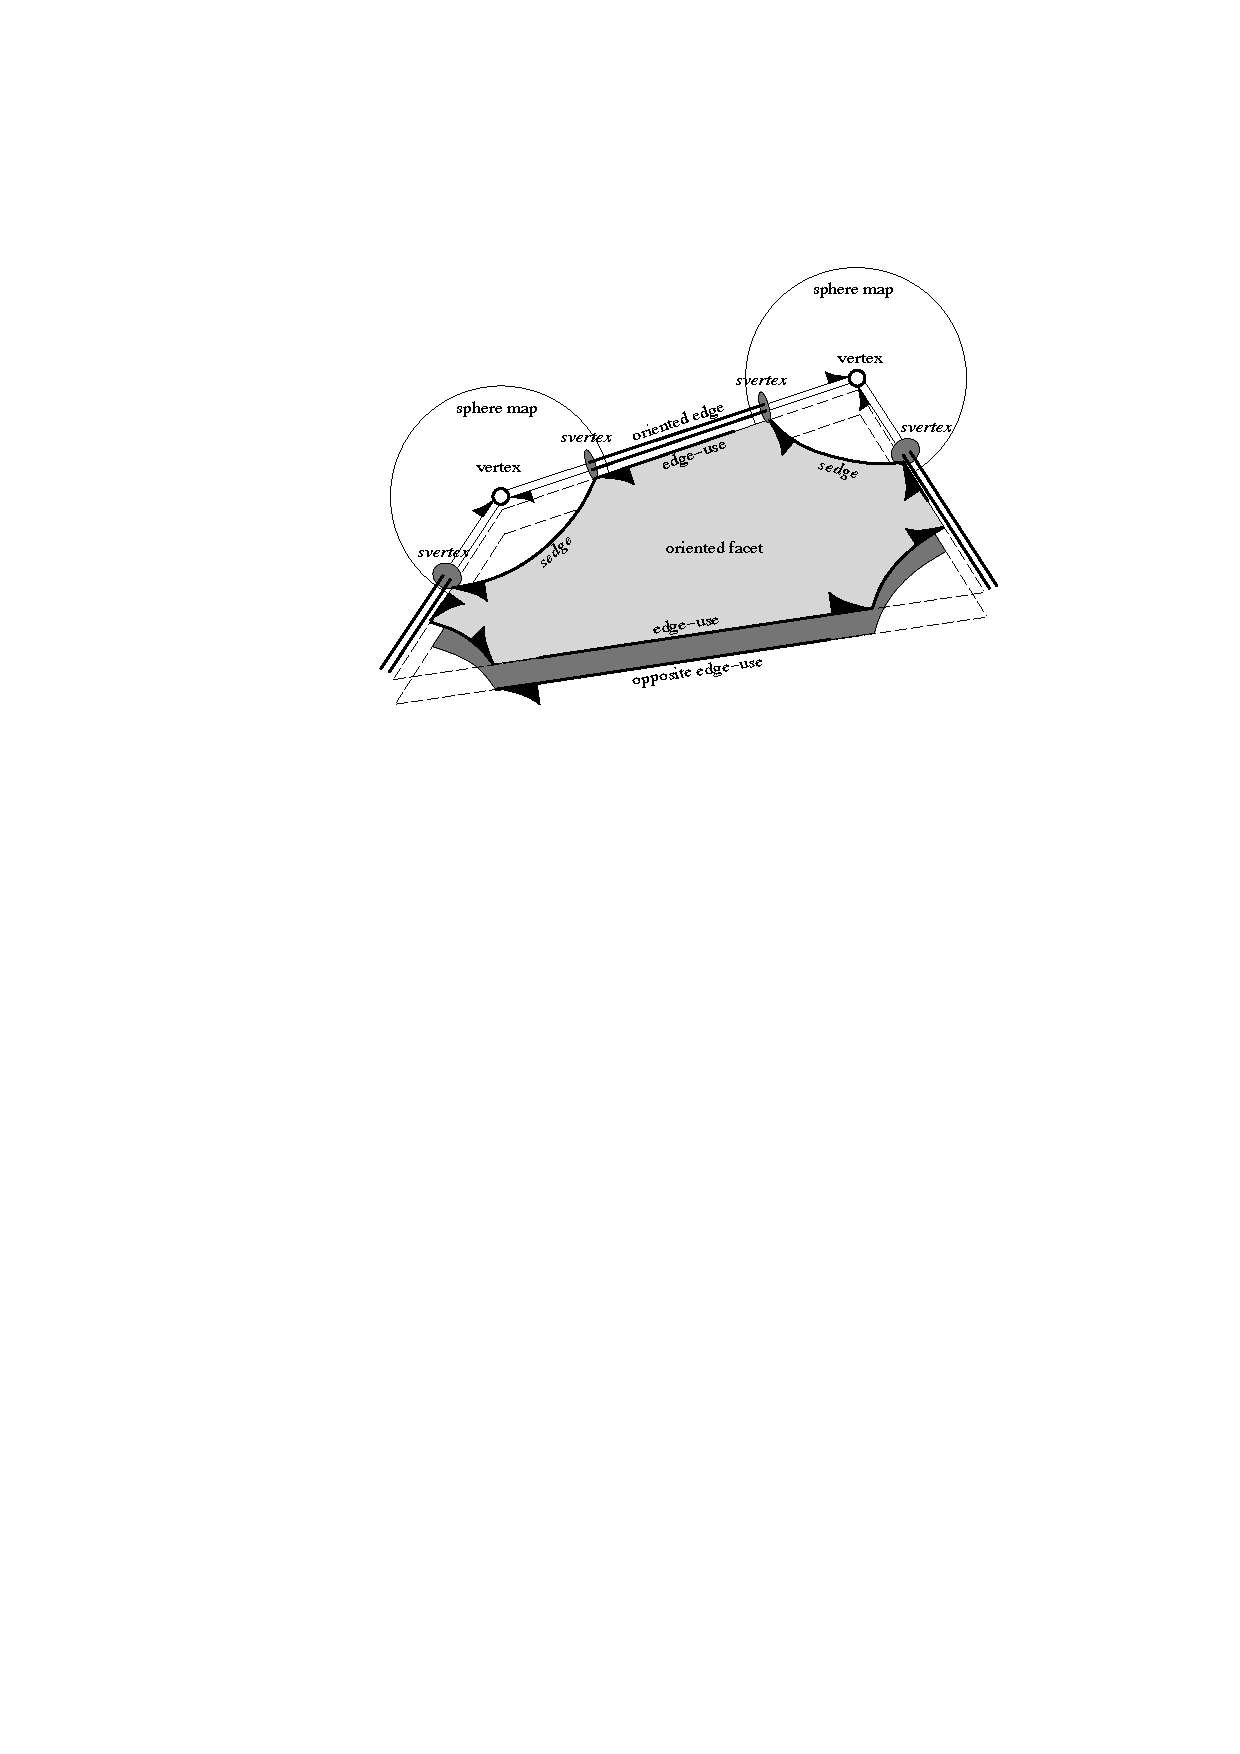
\includegraphics[width=\linewidth]{figs/snc}
\caption{A selective Nef complex.
The standard half-edge structure on 3D space uses faces (as an oriented facet for each incident polyhedron), edges (as an edge-use for each incident oriented facet) and vertices.
The half-edge structure on the surfaces of the spheres representing local vertices, known as sphere maps, uses \emph{sfaces} (per incident polyhedron but not shown here), \emph{sedges} (per incident face) and \emph{svertices} (per incident edge).
From \citet{Hachenberger06}.}%
\label{fig:snc}
\end{figure}

Selective Nef complexes (SNC) use a combination of two half-edge data structures:

\begin{itemize}
\item a standard half-edge data structure on 3D space, which stores each face of each polyhedron as a cycle of \emph{edge-uses} connecting vertices;
\item a half-edge data structure to represent each local pyramid (one per vertex) as a subdivision on the surface of an (infinitesimally small) sphere.
\end{itemize}

Each vertex is linked to its sphere map, where each incident volume corresponds to a face on its sphere map (sface), each incident face corresponds to an edge (sedge), and each incident edge corresponds to a vertex (svertex).
These corresponding elements are linked to each other, which makes it possible to navigate both on the half-edge data structure in 3D space (\eg\ by going from an edge-use to the next to cycle around a face) and on the half-edge data structure of a sphere map (\eg\ by going from one sedge to the next to cycle around an sface).

%%%
%
\section{Exercises}

\begin{enumerate}
	\item How can you define a cube using:
	\begin{enumerate}
		\item a parametric representation
		\item a b-rep data structure
		\item an intersection of half-spaces
	\end{enumerate}
	\item In the line \(L = a p_1 + (1-a) p_2 \), what is the geometry given by \(a < 0\) and \(a > 1\)?
	\item Compute the ranges for the local pyramids of some other vertices in 
	\reffig{nef-boolean}.
	\item In which cases is simplification needed in 2D\@?
	\item Imagine the voxel CSG engine briefly mention in \refsec{psetops}. What would you use for leaf nodes in the CSG tree? How would you implement Boolean set operations on them?
\end{enumerate}



%%%
%
\section{Notes and comments}

If you need more help with the mathematical background, check the Wikipedia pages on sets\footnote{\url{https://en.wikipedia.org/wiki/Set_(mathematics)}}, set algebra\footnote{\url{https://en.wikipedia.org/wiki/Algebra_of_sets}}.

The earliest description of CSG is likely \citet[\S{}12.3]{Requicha77} and its properties is \citet{Requicha78}.
However, it is more of a culmination of efforts of many people.
For instance, \citet{Shamos76} and \citet{Preparata79} show that it is possible to represent any convex object (of any dimension) as the intersection of a finite number of half-spaces.
In order to see how such a decomposition can be done, see \citet{Chazelle79} or \citet{Bajaj90}.
A nice example of how half-spaces can be stored in practice is \citet{Naylor90}.

Nef polyhedra were originally described in \citet{Nef78}, although a much better description including the way they work with Boolean set operations is available in \citet{Bieri88}.

For more background on the line arrangement problem, see the relevant Wikipedia page\footnote{\url{https://en.wikipedia.org/wiki/Arrangement_of_lines}}.
For a clear description of how to compute one, see \citet[\S{}2]{deBerg08} or the user manual of the \texttt{Arrangements\_2} package of CGAL\footnote{\url{https://doc.cgal.org/latest/Arrangement_on_surface_2/index.html}}.

Nef polyhedra as a CSG engine in practice is only possible thanks to \citet{Seel01} in 2D and \citet{Hachenberger06} in 3D.
They discuss how to compute local pyramids in 2D and 3D, as well as Boolean point set operations on polygons and polyhedra.
They are implemented in the CGAL packages 2D Boolean Operations on Nef Polygons\footnote{\url{https://doc.cgal.org/latest/Nef_2/index.html}} and 3D Boolean Operations on Nef Polyhedra\footnote{\url{https://doc.cgal.org/latest/Nef_3/index.html}}.

The general scheme to perform geometric operations in three steps (subdivision, selection and simplification) is discussed by \citet{Rossignac89}.
 % 4.2
% %!TEX root = ../3dchapter.tex

\setchapterpreamble[u]{\margintoc}

\graphicspath{{gmaps/}}
\renewcommand*{\thelesson}{5.1}

\chapter{Generalised and combinatorial maps}%
\label{chap:gmaps}

Generalised maps and combinatorial maps are two related data structures to represent objects of any dimension using a single consistent definition.
2D combinatorial maps are basically the same as most half-edge data structures, with the minor difference that the links between primitives are defined in a manner that works consistently in every dimension.
However, they have clear advantages when we move to 3D combinatorial maps, in which we can break the limits of boundary representation and can store links between adjacent volumes.

As for generalised maps, they are very similar to the combinatorial maps of the same dimension, but they avoid the concept of orientation at the cost of having twice as many primitives.
Theoreticians thus mostly focus on how generalised maps can represent unorientable objects.
However, the most interesting aspect about them is that by omitting orientation, they make building many algorithms easier.

Higher-dimensional generalised and combinatorial maps (\ie\ 4D and higher) can be used to incorporate other non-spatial features, such as time and scale, although this is more of a research topic than a practical application.

\section{What are generalised and combinatorial maps?}

\emph{Generalised maps} (\emph{g-maps}) and \emph{combinatorial maps} (\emph{c-maps} or just \emph{maps}) are what are known as \emph{ordered topological models}.
These are subdivisions of space into abstract simplices (Figure~\ref{fig:simplices}), much like a geometric triangulation in 2D or a tetrahedralisation in 3D.
However, unlike the latter, the subdivision operation to create an ordered topological model is a purely combinatorial operation, \ie\ no geometric tests are ever made.

\begin{figure}
\centering
\includegraphics[width=0.5\linewidth]{figs/simplex}
\caption{An \(n\)-dimensional simplex, or simply \(n\)-simplex, is a combinatorial primitive made from a set of \(n+1\) vertices.
A 0-simplex is thus a point, a 1-simplex is a line segment, a 2-simplex is a triangle, and a 3-simplex is a tetrahedron.
Here they are shown as if embedded in 3D space (\ie\ \(\mathbb{R}^3\)).}%
\label{fig:simplices}
\end{figure}

At this point, it is very important to note that the simplices in an ordered topological model \emph{do not correspond to actual simplices in space}, \ie\ they do not represent actual triangles or tetrahedra that you can point to in a 3D model.
However, there are a few geometric interpretations that are possible, and we will be using one of them to help in understanding, but please bear in mind that it is slightly incorrect from a theoretical standpoint.

\subsection{Darts}

The most precise geometric interpretation is as follows: a generalised or combinatorial map is akin to a barycentric triangulation.
Shortly, a barycentric triangulation of a polygon is a simple way to triangulate a roughly convex polygon by adding a new vertex at its barycentre, then creating new triangles by joining this new vertex to every existing edge in the triangulation, \ie\ forming new triangles with the two vertices on the ends of every existing edge plus the new vertex at the barycentre.
This method creates more triangles than are absolutely necessary in a triangulation, but it does so without doing any geometric tests (unlike a constrained triangulation).

In a 2D combinatorial map, the triangulation that is performed is similar to what was described above (Figure~\ref{subfig:cmaps-simplices}), with the difference that the new vertex is not really located at the barycentre.
In fact, that vertex is not located anywhere---hence why the simplices created using this process are called \emph{abstract simplices}.
In the figures, we thus place the new vertex in a convenient location that avoids visually overlapping simplices, but this is just an arbitrary choice to make the figures clearer.

In a 2D generalised map, the barycentric triangulation requires an extra step where we first split every edge into two by adding a vertex at their barycentres (which is equivalent to a barycentric 1D triangulation of the edge), and then do the 2D triangulation as described above (Figure~\ref{subfig:gmaps-simplices}).
Note that this means that a generalised map has exactly twice as many simplices as a combinatorial map of the same model.

\begin{figure}
\centering
\begin{subfigure}{0.3\linewidth}
\includegraphics[width=\linewidth]{figs/cmaps-simplices}
\caption{}%
\label{subfig:cmaps-simplices}
\end{subfigure}
\quad
\begin{subfigure}{0.3\linewidth}
\includegraphics[width=\linewidth]{figs/gmaps-simplices}
\caption{}%
\label{subfig:gmaps-simplices}
\end{subfigure}\\
\caption{The barycentric triangulation interpretation of: (a) a 2D combinatorial map and (b) a 2D generalised map}%
\label{fig:maps-simplices}
\end{figure}

Now, this is where the \emph{ordered} part of an ordered topological model comes in.
Every vertex in the simplices that were created can be associated with an element of a certain dimension.
The original vertices are zero-dimensional, the new vertices on the edges (for g-maps) are one-dimensional, the new vertices on the faces are two-dimensional, and so on.
Doing so reveals that:

\begin{itemize}
\item every simplex in a 2D generalised map has one vertex of every dimension (\ie\ \(0\), \(1\) and \(2\)), and
\item every simplex in a 2D combinatorial map has two zero-dimensional vertices and one two-di\-men\-sio\-nal vertex (\ie\ \(0\), \(0\) and \(2\)).
\end{itemize}

In order to get the tetrahedralisation for a 3D generalised or combinatorial map, we start from the triangulation describing the 2D generalised or combinatorial map of every face, and then we tetrahedralise by adding a new vertex in the barycentre of each volume.
This new vertex is connected to every existing triangle to form the new tetrahedra, which follow the same ordering pattern as before (Figure~\ref{fig:cmap-3d}).
Formulating it in a dimension-independent way, we have that:

\begin{figure}
\centering
\begin{subfigure}{0.33\linewidth}
\includegraphics[width=\linewidth]{figs/cube}
\caption{}%
\label{subfig:cube}
\end{subfigure}%
\begin{subfigure}{0.33\linewidth}
\includegraphics[width=\linewidth]{figs/cmap-3d}
\caption{}%
\label{subfig:cmap-3d}
\end{subfigure}%
\begin{subfigure}{0.33\linewidth}
\includegraphics[width=\linewidth]{figs/cmap-3d-vertices}
\caption{}%
\label{subfig:cmap-3d-vertices}
\end{subfigure}\\
\caption{(a) A cube, (b) its barycentric tetrahedralisation for a 3D combinatorial map, and (c) one of its simplices showing the ordered property.}%
\label{fig:cmap-3d}
\end{figure}

\begin{itemize}
\item every simplex in an \(n\)D generalised map has one vertex of every dimension up to \(n\) (\ie\ \(0, 1, 2, \ldots, n\)), and
\item every simplex in an \(n\)D combinatorial map has two zero-dimensional vertices and one one vertex of every dimension from \(2\) up to \(n\) (\ie\ \(0, 0, 2, \ldots, n\)).
\end{itemize}

In a generalised or combinatorial map, the primitives that are used to describe the geometry of objects are precisely these \(n\)D abstract simplices, which are called \emph{darts}.

\subsection{Permutations and involutions}

Let us define some properties of \(n\)-simplices that are important for generalised and combinatorial maps.
An \(n\)-simplex can have up to \(n+1\) adjacent other simplices as neighbours, where adjacency is defined as sharing a common \((n-1)\)-simplex on its boundary.
That is, a line segment can have up to two adjacent line segments (each sharing a vertex), a triangle can have up to three adjacent triangles (each sharing an edge), a tetrahedron can have up to four adjacent tetrahedra (each sharing a triangular face), and so on.
Note that these numbers will be lower for the simplices on the boundary of the model.

Therefore, a dart in a 2D generalised/combinatorial map will have up to three neighbouring darts, whereas a dart in a 3D generalised/combinatorial map will have up to four neighbouring darts, and these neighbours will have all but one of the same vertices as the original dart.
Since two adjacent \(n\)-simplices will have a common \((n-1)\)-simplex on their common boundary, going from a dart to its adjacent neighbour will therefore switch only one of its vertices.
Then, since the ordered property tells us the exact combination of dimensional elements that any simplex must have, the switch must exchange an element of a certain dimension for another element of the same dimension (while keeping all of the other previous elements).

In a generalised map, the operation to change the \(0\)-dimensional element, known as \(\alpha_0\), will thus switch a vertex for another vertex on the same edge, face and volume.
Similarly, the operation to change the \(1\)-dimensional element (\(\alpha_1\)) will switch an edge for another edge on the same vertex, face and volume, the operation to change the \(2\)-dimensional element (\(\alpha_2\)) will switch a face for another face on the same vertex, edge and volume, and the operation to change the \(3\)-dimensional element (\(\alpha_3\)) will switch a volume for another volume on the same vertex, edge and face.
These are thus all denoted as \(\alpha_i\), where \(i\) is the dimension of the element being switched.

In a combinatorial map, the operations are slightly different because of the two \(0\)-dimensional elements, which means that changing either \(0\)-dimensional element will switch an \emph{edge} for either of its two adjacent edges.
Since having an operation that yields two different results is undesirable, we therefore have to choose one of these edges as a result of the operation, which means giving the combinatorial map an \emph{orientation} (Figure~\ref{fig:cmaps-orientation}).
This orientation is defined by ordering the two \(0\)-dimensional elements in the dart, and as in half-edge data structures, two darts connected by an involution should have \emph{opposite orientations}.
Since this operation switches the edges of a dart, it is thus denoted as \(\beta_1\).
As for the other operations, they are defined as in a generalised map, but they are all denoted as \(\beta_i\), where \(i\) is the dimension of the element being switched.

\begin{figure}
\centering
\begin{subfigure}{0.33\linewidth}
\includegraphics[width=\linewidth]{figs/cmaps-orientation-1}
\caption{}%
\label{subfig:cmaps-orientation-1}
\end{subfigure}%
\quad
\begin{subfigure}{0.33\linewidth}
\includegraphics[width=\linewidth]{figs/cmaps-orientation-2}
\caption{}%
\label{subfig:cmaps-orientation-2}
\end{subfigure}\\
\caption{Every connected component in a combinatorial map has two possible orientations.
Here, the arrows are darts.
Note how a 2D combinatorial map is equivalent to a half-edge data structure.}%
\label{fig:cmaps-orientation}
\end{figure}

While the triangulation analogy is useful, visually representing darts as simplices is cumbersome and it does not work well in 3D.
For example, consider how the tetrahedra in Figure~\ref{subfig:cmap-3d} visually obstruct each other, which means that showing a more complex polyhedron than a cube is not ideal.
Because of this, most visualisations of generalised maps and combinatorial maps skip the vertices for 2-dimensional elements and higher, resulting in something that looks like a half-edge data structure (Figure~\ref{fig:2dcc}).

\begin{figure}
\centering
\begin{subfigure}{0.33\linewidth}
\includegraphics[scale=0.7]{figs/2dcc}
\caption{}%
\label{subfig:2dcc}
\end{subfigure}%
\quad
\begin{subfigure}{0.33\linewidth}
\includegraphics[scale=0.7]{figs/2dcc-gmap}
\caption{}%
\label{subfig:2dcc-gmap}
\end{subfigure}\\
\begin{subfigure}{0.33\linewidth}
\includegraphics[scale=0.7]{figs/2dcc-alphas}
\caption{}%
\label{subfig:2dcc-alphas}
\end{subfigure}%
\quad
\quad
\begin{subfigure}{0.33\linewidth}
\includegraphics[scale=0.7]{figs/2dcc-betas}
\caption{}%
\label{subfig:2dcc-betas}
\end{subfigure}\\
\caption{(a) Three polygons, (b) their simplices while represented as a 2D generalised map, and alternative geometric interpretations of them as (c) a 2D generalised map and (d) a combinatorial map.}%
\label{fig:2dcc}
\end{figure}

Except for the special case of \(\beta_1\), it is important to note that applying the operation to switch from a dart to its neighbour twice results in returning to the same dart.
Since such an operation is equal to its own inverse, it is known mathematically as an \emph{involution}.
As for \(\beta_1\), it forms a loop of darts around a face that eventually returns to the original dart, and it is thus known instead as a \emph{permutation}.

\subsection{Orbits and sewing}

Starting from a given dart \(d\), the operation to obtain all the darts connected to it while following only the permutations/involutions corresponding to certain dimensions is known as an \emph{orbit} of \(d\).

Among these orbits, the most important one is the one to obtain all the darts belonging to a particular \emph{cell}, \ie\ a vertex, edge, face, or volume.
As we discussed previously, changing the \(i\)-dimensional cell (\(i\)-cell) of a dart, \ie\ applying \(\alpha_i\) or \(\beta_i\), means switching to an adjacent \(i\)-cell.
By the opposite logic, the orbit that obtains all the darts of an \(i\)-dimensional cell is the one that follows all the permutations and involutions except for \(\alpha_i\) or \(\beta_i\) (Figure~\ref{fig:darts-of-cell}).
For an \(n\)-dimensional generalised map, we can denote this as \(\langle \alpha_0, \ldots, \alpha_{i-1}, \alpha_{i+1}, \ldots, \alpha_n \rangle(d)\), and for an \(n\)-dimensional combinatorial map, we can denote this as \(\langle \beta_1, \ldots, \beta_{i-1}, \beta_{i+1}, \ldots, \beta_n \rangle(d)\).

\begin{figure}
\centering
\begin{subfigure}{0.4\linewidth}
\includegraphics[width=\linewidth]{figs/darts-of-cell-1}
\caption{}%
\label{subfig:darts-of-cell-1}
\end{subfigure}%
\quad
\begin{subfigure}{0.4\linewidth}
\includegraphics[width=\linewidth]{figs/darts-of-cell-2}
\caption{}%
\label{subfig:darts-of-cell-2}
\end{subfigure}\\
\caption{(a) A 3D generalised map of a cube, and (b) the orbits that represent one of its vertices, one of its edges and one of its faces.}%
\label{fig:darts-of-cell}
\end{figure}

Note that this means that the objects of any dimension are thus defined as \emph{sets of darts}.
While this is normal for faces and volumes in most other data structures, this applies also to vertices and edges in generalised and combinatorial maps.

Another important orbit is the one that obtains all the darts belonging to an \(i\)-cell within a \(j\)-cell, where \(i < j\).
This can be obtained using the orbit that follows all the permutations and involutions up to \(j-1\) except for \(\alpha_i\) or \(\beta_i\).
For instance, the darts belonging to an edge within a single volume (without obtaining the darts of the same edge but on other volumes) are obtained as \(\langle \alpha_0, \alpha_2 \rangle(d)\) in a generalised map and \(\langle \beta_2 \rangle(d)\) in a combinatorial map.

An important characteristic of orbits is that if they are implemented with some care, it is possible to use them to iterate over the darts of a cell in a consistent order.
This is the basis of the operation that is used to construct generalised and combinatorial maps, which is called \emph{sewing}.
In order to sew together two \(i\)-dimensional objects, the \(i\)-sewing operation starts from two corresponding darts on a common (\(i-1\))-cell but on different \(i\)-cells (Figure~\ref{fig:3-sew}).
It then proceeds to do a parallel traversal of each of their (\(i-1\))-orbits while connecting corresponding darts with \(\alpha_i\) (for a g-map) or \(\beta_i\) (for a c-map).

\begin{figure}
\centering
\includegraphics[width=0.8\linewidth]{figs/3-sew}
\caption{A 3-sewing operation to connect two cubes along a common face.
Note that the operation should start from corresponding darts on either volume.}%
\label{fig:3-sew}
\end{figure}

This process can be used to simply connect adjacent \(i\)-dimensional objects together, but it can also be used to create (\(i+1\))-dimensional objects.
For example, two vertices can be 0-sewn to create an edge (in a g-map), adjacent pairs of edges in a loop can be 1-sewn to create a face, a set of faces enclosing a volume can be 2-sewn along their common edges to create a volume.

\section{Implementing generalised and combinatorial maps}

With data structures for geometric modelling, it is often useful to separate them into two parts: (i) a combinatorial structure that describes the primitives and the relationships between them, and (ii) an embedding structure that maps the primitives to space and stores additional information (\eg\ attributes).
This division is particularly clear in generalised and combinatorial maps.

The most common way to implement a generalised or combinatorial map encodes each dart as a pair of tuples: one for the combinatorial part and one for its embedding.
The combinatorial tuple contains all the permutations and involutions of the dart in order according to their dimension.
For instance, these can be pointers or memory addresses of other darts, or something like ids (in which case the tuple should also contain an id for the dart).
When no objects are connected to a dart through that permutation/involution, a special marker can be used (\eg\ null or zero).

As for the embedding tuple, it generally consists of links to specific structures to store the geometry and attributes for the cell of each dimension that a dart belongs to.
For example, the first element of the tuple could then be a link to a 0-embedding structure, which then contains a list of attributes about the vertex of that dart, the next element could be a link to a 1-embedding structure with information about its edge, and so on.
If no embedding information is needed for the cells of a particular dimension, the corresponding item in the tuple can be omitted, although it is generally desirable to have at least a basic embedding structure with an id.

Regarding the geometric information, in the simplest case, where all geometries are linear (\ie\ line segments, polygons and polyhedra), the 0-embedding structure of a particular vertex can just contain its point coordinates.
From these points, we can linearly interpolate the higher-dimensional geometries by assuming that line segments connect two points and polygons are bounded by (roughly coplanar) line segments.
This kind of data structure with the linear geometries assumption is known as a \emph{linear cell complex}.

More complex geometries can be however stored in a generalised or combinatorial map using the higher-dimensional embeddings.
For instance, we can store the control points for a B\'ezier curve in its 1-embedding structure, or the ones for a B\'ezier surface in its 2-embedding structure.

%%%
%
\section{Exercises}

\begin{enumerate}
	\item Why do barycentric triangulations only work well with roughly convex polygons/polyhedra?
	\item Look at the differences between g-maps and c-maps. Can you tell why implementing algorithms on c-maps is often much harder than on g-maps?
	\item What are the equivalent operations between the DCEL and a 2D combinatorial map?
	\item Rather than storing links to special embedding structures for each dimension in the embedding tuple of a dart, it is also possible to store point coordinates directly. Why is this usually a bad idea?
\end{enumerate}



%%%
%
\section{Notes and comments}

\(n\)-dimensional generalised and combinatorial maps were developed by \citet{Lienhardt94} as a generalisation of 2D combinatorial maps~\citep{Edmonds60}.
Independently, the cell-tuple structure~\citep{Brisson89} was developed as a generalisation of the quad-edge \citep{Guibas85} data structure in 2D and the facet-edge data structure \citep{Dobkin87} in 3D.
The two data structures (generalised maps and the cell-tuple) are basically equivalent.
However, for a more in-depth look at combinatorial maps, see \citet{Damiand14} instead.

Chains of maps \citep{Elter94} supplement the approach used in generalised maps and combinatorial maps with an incidence graph, which can be used to support non-manifolds, but they are rarely used because of their extremely high space requirements.

Moka\footnote{\url{http://moka-modeller.sourceforge.net}} is a nice free modeller that uses generalised maps.
There are also good implementations of generalised maps\footnote{\url{https://doc.cgal.org/latest/Generalized_map/index.html}} and combinatorial maps\footnote{\url{https://doc.cgal.org/latest/Combinatorial_map/index.html}} in CGAL\@.
 % 5.1
% %!TEX root = ../3dchapter.tex

\setchapterpreamble[u]{\margintoc}

\graphicspath{{mat/}}
\renewcommand*{\thelesson}{5.2}

\chapter{The Medial Axis Transform}%
\label{chap:mat}

The Medial Axis Transform (MAT) is yet another way to represent a 3D model.
It can be considered a \emph{dual} representation to the b-rep, similar to how the Voronoi diagram is dual to the Delaunay triangulation. 
Contrary to the b-rep, that represents a model by describing explicitly its boundary surface, the MAT describes a model by its \emph{skeleton} (compare Figures~\ref{fig:gbm:brep} and \ref{fig:gbm:maxis}).
Both the MAT and the b-rep contain exactly the same information and it is possible to convert one to the other without loss of information.

Compared to other shape representations, this skeleton structure makes different properties of the model explicit.
For example, the MAT allows us to split a shape into parts simply by looking at the branches of the skeleton. 
The resulting shape parts often turn out to be meaningful in practice. 
Observe for instance that for the gingerbread man in Figure~\ref{fig:gingerman}, its arms, legs, torso and head each have one corresponding branch in its medial axis (compare Figures~\ref{fig:gbm:whole} and \ref{fig:gbm:maxis}).
For DTMs for example, equally meaningful decompositions into parts can be made, \eg\ the MAT allows us to decompose a DTM into separate hills, watercourses and other objects on top the DTM (see Figure~\ref{fig:matterrain}).

\section{Defining the MAT}
The MAT can be computed both for 2D and 3D objects (compare Figures~\ref{fig:3dmat_2d} and~\ref{fig:3dmat_halfopen}).
\begin{figure}
	\centering
	\begin{subfigure}[b]{0.25\linewidth}
		\centering
		\includegraphics[width=\textwidth]{figs/gingerbreadman_whole.pdf}
		\caption{A 2D object}
		\label{fig:gbm:whole}
	\end{subfigure}
	\qquad%
	\begin{subfigure}[b]{0.25\linewidth}
		\centering
		\includegraphics[width=\textwidth]{figs/gingerbreadman_brep.pdf}
		\caption{b-rep}
		\label{fig:gbm:brep}
	\end{subfigure}
	\qquad%
	\begin{subfigure}[b]{0.25\linewidth}
		\centering
		\includegraphics[width=\textwidth]{figs/gingerbreadman_skeleton.pdf}
		\caption{Interior MAT}
		\label{fig:gbm:maxis}
	\end{subfigure}
	
	\begin{subfigure}[b]{0.3\linewidth}
		\centering
		\includegraphics[width=\textwidth]{figs/gingerbreadman_mat.pdf}
		\caption{b-rep + MAT with medial balls}
		\label{fig:gbm:mballs}
	\end{subfigure}
	\qquad
	\begin{subfigure}[b]{0.3\linewidth}
		\centering
		\includegraphics[width=\textwidth]{figs/gingerbreadman_grassfire.pdf}
		\caption{b-rep + contours of equal distance to it + MAT}
		\label{fig:gbm:dt}
	\end{subfigure}
	
	\caption{Different ways to represent the shape of gingerbread man}
	\label{fig:gingerman}
\end{figure}
\begin{figure}
	\centering
	\begin{subfigure}{0.26\linewidth}
		\includegraphics[width=\linewidth]{figs/Box2D3D/3dmat_2d.pdf}
		\subcaption{The MAT for a 2D box consists of medial balls (blue) and the medial axis (red).}
		\label{fig:3dmat_2d}
	\end{subfigure}
	\quad
	\begin{subfigure}{0.33\linewidth}
		\includegraphics[width=\linewidth]{figs/Box2D3D/3dmat_halfopen.png}
		\subcaption{3D medial balls of a 3D box shape.}
		\label{fig:3dmat_halfopen}
	\end{subfigure}
	\quad
	\begin{subfigure}{0.33\linewidth}
		\includegraphics[width=\linewidth]{figs/Box2D3D/3dmat_sheets.png}
		\subcaption{3D medial axis of a 3D box shape.}
		\label{fig:3dmat_sheets}
	\end{subfigure}
	\caption{The MAT in 2D and in 3D for a box shape.}
	\label{fig:3dmat}
\end{figure}
In both cases there are two equivalent definitions of the MAT\footnote{Sometimes the MAT is referred to as medial axis function, stick figure, skeleton or surface skeleton.
	Inventor Harry Blum finally settled on symmetry axis, as he considered symmetry to be the crucial role of the MAT \citep{Blum73}.} that apply. 
One is based on the distance transform, and one is based on medial balls. 
Both definitions describe how to obtain the MAT from the boundary, denoted $
\mathcal{B}$ of an object (Figure~\ref{fig:gbm:brep}).
And both can be applied to both 2D and 3D objects .

\begin{description}
	\item[Grassfire analogy]
	Imagine that everything is made of grass and that all the points on $\mathcal{B}$ are simultaneously set on fire at time $t=0$. 
	The fire spreads evenly to all directions at constant speed. 
	Now, the MAT is defined as the set of points where the fire front meets itself. 
	This concept is illustrated in Figure~\ref{fig:gbm:dt}, where each contour can be seen as a fire front at some constant time $t$. The medial axis is drawn where the fire front meets itself.
	\item[Medial balls]
	A \emph{medial ball} is a ball that fits completely inside $\mathcal{B}$ and does not contain any other ball that would fit inside $\mathcal{B}$. 
	The MAT is defined as the set of points that are the centres of all medial balls of $\mathcal{B}$ (see Figure~\ref{fig:gbm:mballs}). 
	Notice that each medial ball touches $\mathcal{B}$ in at least two points, called its \emph{feature points}. 
\end{description}

%TODO: that should also be in the figure
As illustrated in Figure~\ref{fig:gbm:maxis}, the MAT can be subdivided into \emph{medial branches} and \emph{junctions}. 
Junctions are locations where three or more medial branches coincide. 
The points of the MAT are called \emph{medial atoms}, or simply \emph{atoms}. 
Observe that if an atom has exactly two feature points, it is part of a medial branch, and if it has more than two feature points it lies on a junction or on the tip of a medial branch. 
The medial branches, its junctions and how those are are connected define the \emph{medial structure}.
% If we consider that each branch corresponds to one part of $\mathcal{B}$ gives us a natural way to split an object into parts

For a 2D object, such as in Figure~\ref{fig:gingerman}, the medial branches are curves and the the junctions are points. 
However, for a 3D object, the medial branches can also be surfaces (see Figure~\ref{fig:3dmat_sheets}), and the junctions can also be curves.
The branches of the 3D MAT are therefore also called \emph{medial sheets}.

\subsection{Medial geometry}
The medial geometry describes how atoms are related to the object boundary $\mathcal{B}$. 
It is defined for each medial atom that is part of a medial sheet. 
Figure~\ref{fig:medialgeometry} illustrates the complete medial geometry of an atom.
The medial ball $B$ has the atom $\mathbf{c}$ at its center and has a radius $r$, \ie\ the shortest distance from $\mathbf{c}$ to $\mathcal{B}$.
The medial ball $B$ touches the boundary $\mathcal{B}$ at the feature points $\mathbf{p}$ and $\mathbf{q}$.
The vectors from $\mathbf{c}$ to $\mathbf{p}$ and $\mathbf{q}$ are called the \emph{spoke vectors}, denoted $\vec{\mathbf{s_{p}}}$ and $\vec{\mathbf{s_{q}}}$. 
The angle between the spoke vectors is called the \emph{separation angle}, denoted $\theta$ and the bisector of the spoke vectors is called the \emph{medial bisector}, denoted $\vec{\mathbf{b}}$.

\begin{figure}
	% \centering
	% \setcapindent{1em}
	\centering
	\begin{minipage}[c]{0.4\linewidth}
		\includegraphics[width=\linewidth]{figs/medial_atom_geometry.pdf}
	\end{minipage}
	\begin{minipage}[c]{0.45\textwidth}
		% \hspace{1.1em}
		\centering
		\begin{tabular}{ll}
			\toprule
			Symbol & Description \\
			\midrule
			$B(\mathbf{c},r)$& medial ball\\
			$\mathbf{c}$ & medial atom\\
			$r$ & radius\\
			$\mathbf{p}, \mathbf{q}$ & feature points\\
			$\vec{\mathbf{s_{p}}}, \vec{\mathbf{s_{q}}}$ & spoke vectors\\
			$\theta$ & separation angle\\
			$\vec{\mathbf{b}}$ & medial bisector\\
			\bottomrule
		\end{tabular}
	\end{minipage}
	\caption{The geometry of a medial atom.}
	\label{fig:medialgeometry}
\end{figure}

% maximal/medial ball, primary and secondary feature point, primary and secondary medial ball, separation angle, bisector, medial atom:point+ball+metrics, 
% defining local coordinate system
% \subsection{Properties of the MAT}
Using the medial geometry we can describe a number of interesting properties of the MAT.
\begin{enumerate}
	\item Any atom $\mathbf{c}$ is always \emph{medial} to $\mathcal{B}$, \ie\ it is equidistant to the feature points of $\mathbf{c}$ (hence the name of the MAT).
	\item The medial ball $B$ is always tangential to $\mathcal{B}$ at the feature points. 
	\item The radius $r$ can be used to define the `thickness' of an object, since it measured the distance to the `middle' of the object where the MAT is located.
	% \item From the union of all interior medial balls of an object, its boundary can be reconstructed.
	% \item The medial bisector $\vec{\mathbf{b}}$ always points in the direction of decreasing radius along a medial branch or sheet.
	% \item The feature points of a medial atom at the tip of a medial branch indicate points of minimal of curvature on $\mathcal{B}$. Notice also that the radius of those atoms is inversely proportional to the curvature at its feature points.
\end{enumerate}

\subsection{Exterior MAT and the MAT of a DTM}
The MAT can be divided into an interior part and an exterior part.
So far we have only looked at the \emph{interior MAT}, which consists of medial balls that reside entirely on the inside of an object.
However, in many cases it is also possible to define medial balls that reside entirely on the outside of an object.
That part of the MAT is called the \emph{exterior MAT}.
An object can only have an exterior MAT if the shape of that object is non-convex, since for convex object it is not possible to find exterior medial balls with a finite radius.
% In case of a composition of multiple objects, the interaction between these object can also lead to an exterior MAT, even if all objects are convex.\todo{illustrate that}

The separation between inside and outside is very clear and unambiguous for a an object with a closed boundary such as the gingerbread man of Figure~\ref{fig:gingerman} or for any perfectly manifold boundary.
However, for objects that are not completely closed this separation is less clear, as there could be MAT sheets that connect the interior and exterior parts though holes in the boundary surface.
In some cases with an open boundary a reasonable distinction can still be made.
For example for a DTM we can follow the convention that the `ground side` of the DTM is the interior, and the `sky side' is the exterior, as follows from Figure~\ref{fig:object_earth}.
\begin{figure}
	\centering
	\begin{subfigure}{0.4\linewidth}
		\includegraphics[width=\linewidth]{figs/object_earth.pdf}
		\subcaption{The interior and exterior of a DTM.}
	\label{fig:object_earth}
	\end{subfigure}
	\quad
	\begin{subfigure}{0.57\linewidth}
		\includegraphics[width=\linewidth]{figs/MAT_hierarchy.pdf}
		\subcaption{For a terrain the MAT is typically subdivided into open clusters that correspond to features such as hills, buildings and watercourses in the terrain. Shown here is a vertical cross section of a DTM. Exterior MAT in light blue, interior MAT in dark blue.}
		\label{fig:matterrain}
	\end{subfigure}
	\caption{Defining interior and exterior for an open surface such as a terrain.}
	\label{fig:intext}
\end{figure}
Following this convention, we can still define the interior and exterior MAT of a DTM, see for instance Figure~\ref{fig:matterrain}.

\subsection{Medial clusters}
The interior and exterior MAT can consist of multiple disjoint parts (\eg\ in Figure~\ref{fig:matterrain}).
For closed objects the interior MAT is always one part, whereas the exterior MAT can be multiple parts depending on the number of concavities in the object boundary.
The disjoint parts are called \emph{medial clusters}.
Each medial cluster is in fact a set of adjacent sheet where each adjacency is also a junction between medial sheets.

For objects with open boundaries like DTMs, there can also be multiple interior medial clusters.
In this case one object on the terrain typically corresponds to one medial cluster (Figure~\ref{fig:matterrain}).
Figure~\ref{fig:smat_r3d_int} also illustrates how the MAT can thus be used to meaningfully subdivide an object into parts.
For an input that is simply a surface point cloud that happens to contain several object, we can detect easily these objects by looking at the medial clusters of its MAT.
This effectively decomposes the object into meaningful sub-objects.
\begin{figure}
	\begin{subfigure}[t]{0.45\linewidth}
		\includegraphics[width=\linewidth]{figs/smat/smat_r3d_surface.png}
		\subcaption{Surface points.}
		\label{fig:smat_r3d_surface}
	\end{subfigure}
	\quad
	\begin{subfigure}[t]{0.45\linewidth}
		\includegraphics[width=\linewidth]{figs/smat/smat_r3d_mat.png}
		\subcaption{Medial atoms coloured by medial radius using a repeating colourmap.}
		\label{fig:smat_r3d_mat}
	\end{subfigure}
	\quad
	\begin{subfigure}[t]{0.45\linewidth}
		\includegraphics[width=\linewidth]{figs/smat/smat_r3d_thetad_all.png}
		\subcaption{Medial sheet segmentation.}
		\label{fig:smat_r3d_sheets_all}
	\end{subfigure}
	\quad
	\begin{subfigure}[t]{0.45\linewidth}
		\includegraphics[width=\linewidth]{figs/smat/smat_r3d_ballo_all.png}
		\subcaption{Medial cluster segmentation.}
		\label{fig:smat_r3d_ballo_all}
	\end{subfigure}
	\quad
	\begin{subfigure}[t]{0.45\linewidth}
		\includegraphics[width=\linewidth]{figs/smat/smat_r3d_mat_int.png}
		\subcaption{Interior medial clusters.}
		\label{fig:smat_r3d_ballo_int}
	\end{subfigure}
	\quad
	\begin{subfigure}[t]{0.45\linewidth}
		\includegraphics[width=\linewidth]{figs/smat/smat_r3d_surface_int.png}
		\subcaption{Surface points corresponding to interior medial clusters.}
		\label{fig:smat_r3d_surface_int}
	\end{subfigure}
	\caption{Interior MAT part in.}
	\label{fig:smat_r3d_int}
\end{figure}

% \begin{figure}
% 	\centering
% 	\begin{subfigure}{0.45\linewidth}
% 		\centering
% 		\includegraphics[width=\textwidth]{figs/watercourse_crossec_mat.pdf}
% 		\subcaption{Cross section of a watercourse. The 3D skeleton is obtained by reconstructing medial balls that touch the ground surface in two points.}\label{fig:crosssec}
% 	\end{subfigure}
% 	\qquad
% 	\begin{subfigure}{0.45\linewidth}
% 		\centering
% 		\includegraphics[width=\textwidth]{figs/watercourse_3d_mat.pdf}
% 		\subcaption{Perspective view of the 3D skeleton of simple watercourses.}\label{fig:crosssec3d}
% 	\end{subfigure}
% 	\caption[MAT segmentation]{Profile view of 3D skeleton of the terrain}
% 	\label{fig:MAT2D3D}
% \end{figure}

\section{Computing the MAT} 
Computing the MAT from the boundary $\mathcal{B}$ of an object is typically done in two steps. 
During the first step, \ie\ \emph{MAT approximation}, a noisy approximation of the MAT is obtained, and during the second step, \ie\ \emph{pruning}, the noise is removed.

\subsection{MAT approximation}
The MAT can be approximated in various ways, \eg~by using voxels and distance transforms or as a subset of the Voronoi diagram.
In this lesson, however, we will focus on the so-called shrinking-ball algorithm.

\subsubsection{The shrinking-ball algorithm}
The shrinking-ball algorithm works well for robustly approximating the MAT of 3D objects that are represented using boundary points, \ie point clouds.
It is a simple and fast algorithm that can be made robust to noise in the boundary points.
%This means that pruning the MAT after approximation is not necessary with the shrinking-ball algorithm.
The shrinking-ball algorithm takes an \emph{oriented point cloud} as input, \ie\ a point cloud that includes a normal vector for each point. 
It outputs a disjoint set of medial atoms. 

The algorithm is based on the observation that the medial atom corresponding to a boundary point $\mathbf{p}$ must be positioned somewhere on the line $L$ through the normal $\vec{\mathbf{n}}$ of $\mathbf{p}$.
This observation is used to restrict the search space for the medial ball of $\mathbf{p}$ to the line $L$.
As illustrated by Figure~\ref{fig:shrinkballAlgo}, the algorithm begins with a very large candidate ball for $\mathbf{p}$ that is centered on $L$.
\begin{figure}[tbp]
	\begin{subfigure}{0.245\linewidth}
		\includegraphics[width=\textwidth]{figs/fullBallShrink_1.pdf}
		\subcaption{Initial ball}
		\label{fig:fullBallShrink_1}
	\end{subfigure}
	\begin{subfigure}{0.245\linewidth}
		\includegraphics[width=\textwidth]{figs/fullBallShrink_2.pdf}
		\subcaption{Second iteration.}
		\label{fig:fullBallShrink_2}
	\end{subfigure}
	\begin{subfigure}{0.245\linewidth}
		\includegraphics[width=\textwidth]{figs/fullBallShrink_3.pdf}
		\subcaption{Third iteration.}
		\label{fig:fullBallShrink_3}
	\end{subfigure}
	\begin{subfigure}{0.245\linewidth}
		\includegraphics[width=\textwidth]{figs/fullBallShrink_4.pdf}
		\subcaption{Fourth iteration.}
		\label{fig:fullBallShrink_4}
	\end{subfigure}
	\caption{Ball shrinking iterations with the shrinking-ball algorithm. The final iteration yields a \emph{medial} ball. A legend is given in \subref{fig:fullBallShrink_2}.}
	\label{fig:shrinkballAlgo}
\end{figure}
At each consecutive iteration, a new candidate ball is constructed that is smaller than the previous one and closer to the final \emph{medial} ball.
Every ball is constructed so that it touches $\mathbf{p}$ and is centred on $L$.
Only the candidate feature point $\mathbf{q}$ changes with each iteration.
A new $\mathbf{q}$, denoted $\mathbf{q_{next}}$, is found by selecting the closest point from the centre $\mathbf{c}$ of the current ball.
Using $\mathbf{p}, \vec{\mathbf{n}}, \mathbf{q_{next}}$ we can compute the centre of the next ball $\mathbf{c_{next}}$, at which point we move on to the next iteration.
The algorithm terminates when an empty ball is found, which is the case when the radius no longer shrinks.
Algorithm~\ref{alg:shrinkBall} gives the pseudo-code for the shrinking-ball algorithm.
\begin{algorithm}[tb]
	\SetKwInOut{Input}{Input}
	\SetKwInOut{Output}{Output}
	\DontPrintSemicolon\Input{
		a KD-tree of the surface point cloud $T$,\\ 
		a surface point $\mathbf{p}$\\ 
		it's normal vector $\vec{\mathbf{n}}$, and\\
		the initial ball radius $r_{init}$}
	\Output{the medial ball centre $\mathbf{c}$,\\the medial ball radius $r$}
	$r \leftarrow r_{init}$ \\
	$\mathbf{c} \leftarrow$ the centre of the ball that touches $\mathbf{p}$ is centered on $\vec{\mathbf{n}}$ with a radius $r$ \\
	\Repeat{a \textbf{break} statement is executed} {
		$q_{next} \leftarrow$ the nearest point to $\mathbf{c}$, obtained quickly using $T$ \\
		$r_{next} \leftarrow$ radius of the next ball that touches $\mathbf{p}$ and $\mathbf{q_{next}}$ and is centred on $\vec{\mathbf{n}}$ \\
		$\mathbf{c_{next}} \leftarrow$ centre of the next ball, can be computed with $\mathbf{p}, \vec{\mathbf{n}}$, and $r_{next}$ \\
		\If{$r_{next} = r$} {
			\textbf{break}
		}
		$\mathbf{c} \leftarrow \mathbf{c_{next}}$ \\
		$r \leftarrow r_{next}$
	}
	\caption{The shrinking-ball algorithm.}
	\label{alg:shrinkBall}
\end{algorithm}

The algorithm is run for each point in the input point cloud. 
If the normal vectors point away from the interior, the interior MAT is computed.
And by flipping the orientation of the normal vector, the exterior MAT can also be computed.
If normals are not available for a point cloud, these can be estimated using local plane fitting, \ie\ by fitting a plane to the $k$ nearest neighbours of each boundary point. 
The vector perpendicular to that plane then becomes the estimated normal vector.
A KD-tree is typically used to speed up the nearest neighbour searches, both for normal estimation and the shrinking-ball algorithm.
Figure~\ref{fig:ca_ridge} gives an example result of the shrinking-ball algorithm for a terrain point cloud. 
Observe how the MAT describes the valleys (exterior MAT) and ridges (interior MAT) in the terrain with its skeletal structure.
\begin{figure}
	\centering
	\begin{subfigure}{0.310\linewidth}
		\includegraphics[angle=90,width=\linewidth]{figs/iMAT.png}
		\caption{Interior MAT.}
		\label{fig:ca_ridge:imat}
	\end{subfigure}
	\quad
	\begin{subfigure}{0.310\linewidth}
		\includegraphics[angle=90,width=\linewidth]{figs/terrain.png}
		\caption{Terrain points}
		\label{fig:ca_ridge:terrain}
	\end{subfigure}
	\quad
	\begin{subfigure}{0.310\linewidth}
		\includegraphics[angle=90,width=\linewidth]{figs/oMAT.png}
		\caption{Exterior MAT}
		\label{fig:ca_ridge:omat}
	\end{subfigure}
	\caption{MAT approximation (a,c) of a lidar terrain point cloud (b) obtained with the shrinking-ball algorithm. Top view.}
	\label{fig:ca_ridge}
\end{figure}

Notice that the shrinking ball algorithm subdivides the output only in an interior and exterior part based on the point normals in the input. 
It is possible to further segment the MAT into for example medial sheets and medial clusters.
This can be achieved for example with a region-growing segmentation algorithm that uses properties of the medial geometry (\eg\ the medial bisector). 
Figures~\ref{fig:smat_r3d_sheets_all} and \ref{fig:smat_r3d_ballo_all} show the result of such a segmentation.

% The main limitation of the shrinking-ball algorithm is that it outputs only an unstructured set of medial atoms, \ie\ there is no distinction between its different medial sheets.% and also the surface of the sheets is not explicitly reconstructed.
% This can be solved by using the medial geometry of the medial atoms.
% Several properties of the medial geometry are locally similar within the same medial sheet.
% With a region-growing algorithm this similarity can be exploited to segment the unstructured medial atoms into medial sheets.
% Especially the medial bisector is useful, \ie\ it is tangential to the medial sheet and it always points in the direction of decreasing radius in a sheet, usually away from junction curves.
% It is thus not only similar within one sheet, but also dissimilar for the different sheets that meet at a junction curve.
% As a result there is little chance that a sheet segment grows into another sheet through a junction curve, leading to well separated sheets (see Figure~\ref{fig:MATmeth}).
% Region-growing can also be used to segment the MAT of a DTM in its different disjoint medial clusters.
% In this case the region-growing condition may be based on a measure for the amount of overlap between nearby medial balls.
% Because, nearby medial balls within one medial cluster are likely to overlap, whereas medial balls between different clusters are not.

\subsection{Pruning}
Pruning is the process of retracting or removing unimportant branches from the MAT.
It is often necessary because the MAT is unstable, \ie\ it is extremely sensitive to small bumps in $\mathcal{B}$.
As illustrated in Figures~\ref{fig:mat-instability} and \ref{fig:imaimp:a}, tiny deviations in $\mathcal{B}$ can lead to big spurious branches in the structure of the MAT.
\begin{figure}
	\centering
	\begin{subfigure}{0.425\linewidth}
		\centering
		\includegraphics[width=\textwidth]{figs/protrudingSheets.pdf}
		\subcaption{Small bumps in the boundary can cause big spurious branches to appear. Object boundary drawn in red, MAT in blue.}\label{fig:mat-bumps}
	\end{subfigure}
	\qquad
	\begin{subfigure}{0.50\linewidth}
		\centering
		\includegraphics[width=\textwidth]{figs/spurious_branches.png}
		\subcaption{Spurious branches can appear in the MAT due to a small amount of noise in the boundary.}
		\label{fig:sb_noise}
	\end{subfigure}
	\caption{Instability of the MAT.}
	\label{fig:mat-instability}
\end{figure}
This is especially problematic when $\mathcal{B}$ has some noise as is the case with the typical DTM.
The resulting MAT can become so distorted by the spurious branches that it becomes hard to distinguish its main medial structure.
The main aim of pruning is to remove these spurious branches.

Most pruning methods are based on properties of the medial geometry. 
Based on these properties, an importance measure for each medial atom is defined, which is then used as a threshold to filter medial atoms. 
The resulting (pruned) MAT is usually a subset of the original MAT. 
Some methods preserve topology, others do not or do so only up to a certain level. 
The main challenge is often selecting the optimal threshold value---a compromise between removing noisy MAT parts and not removing fine detail, \ie\ often the endpoints of good MAT branches are also affected by pruning.
Examples of importance measures for pruning are the separation angle $\theta$ (recall this is the angle between the spoke vectors) and the separation distance $\lambda$, \ie the distance between the two feature points of a medial atom. 
These values are typically low for noisy parts of the MAT.
Figure~\ref{fig:imaimp} gives an example of pruning with the separation distance.
\begin{figure}
	\centering
	\begin{subfigure}{0.4\linewidth}
		\includegraphics[width=\linewidth]{figs/rasterimpl/simple_dtm-gamma1_earthskel_.png}
		\caption{MAT without pruning ($\lambda=0$)}
		\label{fig:imaimp:a}
	\end{subfigure}
	\quad
	\begin{subfigure}{0.4\linewidth}
		\includegraphics[width=\linewidth]{figs/rasterimpl/simple_dtm-gamma1_earthskel.png}
		\caption{Reconstructed object for $\lambda=0$.}
		\label{fig:imaimp:b}
	\end{subfigure}
	
	\begin{subfigure}{0.4\linewidth}
		\includegraphics[width=\linewidth]{figs/rasterimpl/simple_dtm-gamma6_earthskel_.png}
		\caption{MAT with medium pruning ($\lambda=6$)}
		\label{fig:imaimp:c}
	\end{subfigure}
	\quad
	\begin{subfigure}{0.4\linewidth}
		\includegraphics[width=\linewidth]{figs/rasterimpl/simple_dtm-gamma6_earthskel.png}
		\caption{Reconstructed object for $\lambda=6$. Despite the pruned MAT, the corresponding boundary remains almost unchanged.}
		\label{fig:imaimp:d}
	\end{subfigure}
	
	\begin{subfigure}{0.4\linewidth}
		\includegraphics[width=\linewidth]{figs/rasterimpl/simple_dtm-gamma10_earthskel_.png}
		\caption{MAT with strong pruning ($\lambda=10$).}
		\label{fig:imaimp:e}
	\end{subfigure}
	\quad
	\begin{subfigure}{0.4\linewidth}
		\includegraphics[width=\linewidth]{figs/rasterimpl/simple_dtm-gamma10_earthskel.png}
		\caption{Reconstructed object for $\lambda=10$. Notice how the tree is separated from the the ground and that edges have become rounder.}
		\label{fig:imaimp:f}
	\end{subfigure}
	\caption{The effect of different levels of pruning on the MAT.}
	\label{fig:imaimp}
\end{figure}

% Pruning is virtually always performed as a post-process when the MAT is approximated using a grid method or a method based on the Voronoi Diagram, extremely clean inputs excepted.
% The shrinking ball algorithm, on the other hand, can be modified in such a way that its output does not require pruning afterwards.
% The modification boils down to checking during each iteraions the separation angle of the candidate medial ball.
% When the separation angle drops below a threshold, the algorithm is terminated and the current candidate ball is picked as the definitive medial ball for the current boundary point.
% This is illustrated in Figure~\ref{fig:sb_noise}, \ie\ because the separation angle $\theta_{i+1}$ of the next atom is very small, the shrinking ball process is terminated at the current atom $\mathbf{c_i}$.
% Notice that the separation angle became so small because the candidate feature point `jumped' from one side of the boundary to the other side (compare $\mathbf{q_i}$ and $\mathbf{q_{i+1}}$).
% This typically happens in the presence of noisy boundary points, and illustrates why filtering on a low separation angle is effective for pruning.

\section{Notes and comments}
The Medial Axis Transform was originally introduced in 1967 by Harry Blum, a biologist \citep{Blum67}.

\citet{Ma12} introduced the shrinking ball algorithm. \citet{Peters18} explains how to make the algorithm robust so that it can be successfully applied to lidar point cloud inputs and how to obtain a sheet and cluster segmentation using a region-growing approach.


%%%
%
\section{Exercises}

\begin{enumerate}
  \item Draw the medial axis of a 2D box. Then draw the medial bisectors. How could the medial bisector be used to distinguish between the different sheets?
  \item For what closed object the MAT is a single point?
  \item Do think the MAT could help us to detect thick and thin parts of an object? If so, how?
\end{enumerate} % 5.2
% \include{curves/curves} % 6.1
% \include{bim/bim} % 6.2
% \include{conversion/conversion} % 7.1
% \include{apps/apps} % 7.2
%----------------------------------------------------------------------------------------


% \backmatter % Denotes the end of the main document content
% \setchapterstyle{plain} % Output plain chapters from this point onwards

%----------------------------------------------------------------------------------------
% BIBLIOGRAPHY
%----------------------------------------------------------------------------------------

% The bibliography needs to be compiled with biber using your LaTeX editor, or on the command line with 'biber main' from the template directory

% \defbibnote{bibnote}{Here are the references in citation order.\par\bigskip} % Prepend this text to the bibliography
\printbibliography[heading=subbibliography, title=Bibliography] % Add the bibliography heading to the ToC, set the title of the bibliography and output the bibliography note

%----------------------------------------------------------------------------------------
% INDEX
%----------------------------------------------------------------------------------------

% The index needs to be compiled on the command line with 'makeindex main' from the template directory

% \printindex % Output the index

%----------------------------------------------------------------------------------------
% BACK COVER
%----------------------------------------------------------------------------------------

% If you have a PDF/image file that you want to use as a back cover, uncomment the following lines

%\clearpage
%\thispagestyle{empty}
%\null%
%\clearpage
%\includepdf{cover-back.pdf}

%----------------------------------------------------------------------------------------

\end{document}
